The Mini Wheelbot involves a number of challenges, making it an interesting testbed for data-driven, learning-based control algorithms.
We showcase two of such algorithms.
In Sec.~\ref{sec:bo}, we use BO which has become popular for controller tuning in the last decade~\cite{chatzilygeroudis2019survey,paulson2023tutorial, marco2016automatic, calandra2016bayesian, berkenkamp2016safe} and allows us to automatically find excellent balancing controller gains in automated hardware experiments.
In Sec.~\ref{sec:ampc}, we use imitation learning from an expert MPC, also called approximate MPC (see~\cite{gonzalez2023neural} for a recent survey).
Approximate MPC avoids slow online optimization which enables sophisticated nonlinear MPC in fast feedback loops onboard robots~\cite{carius2020mpc,nubert2020safe} even on low-cost hardware~\cite{hose2024parameter}.

\subsection{Tuning Stand-up \& Balancing via Bayesian Optimization}
\label{sec:bo}
BO describes a family of black-box optimization algorithms that can be used for controller tuning based on a few interactions with the real world system~\cite{paulson2023tutorial, marco2016automatic, calandra2016bayesian, berkenkamp2016safe,chatzilygeroudis2019survey}. 
Instead of LQR in~\cite{geist2022wheelbot}, we use BO to tune the gains of the state-feedback controller~(\ref{eqn:feedbackgain}) in a direct, data-driven approach based on rewards collected in real-world experiments.
This is practically motivated: Tuning LQR cost matrices can be unintuitive and for some gain combinations, unmodeled high-frequency oscillations occur that are difficult to avoid through the choice of LQR cost.
In addition to finding excellent balancing controller gains, BO illustrates the advantage of automatic environment resets through the Mini Wheelbot's stand-up maneuvers for learning on episodic tasks.


With BO, we find
\begin{align}\label{eqn:bo}
K^* = \argmax_{K} V(K)
\end{align}
based on (noisy) real-world evaluations of the true objective function~$V(K)$.
We define the objective function to be
\begin{align}
    \label{eqn:bo:cost}
    V(K) = 
        \begin{cases}
        -J_\text{c}, & \text{if crash}, \\
        -\frac{1}{T_\text{BO}}\sum_{t=0}^{T_\text{BO}} \|x(t)\|_{Q_\text{BO}}^2 - w_\text{vib}\cdot J_{\text{vib}}, & \text{else},
        \end{cases}
\end{align}
where~$T_\text{BO}$ is the experiments time horizon. The crash penalty~$J_\text{c}$ is empirically chosen slightly worse than a barely successfull experiment (e.g.,~$J_\text{c}=30$ for the experiment shown in Fig.~\ref{fig:boperformanceimprovement}).
For successful experiments, the objective value consists of the mean squared error over the state deviation from the equilibrium with diagonal weights~$Q_\text{BO}=\text{diag}([0,50,200,0,0.4,0.1,0,\dots]^\top)$.
The additional penalty~$J_\text{vib}$ weighted by~$w_\text{vib}=10^{-5}$ is
\begin{align}
    \label{eqn:bo:costvib}
    J_{vib} 
    = \sum_{t=1}^{T_\text{BO}} 
    ( 
        &|\Delta\dot{\phi}(t)|,
        \text{if}\; |\Delta\dot{\phi}(t)| \geq \alpha, \;
        \text{else}\; 0
    ),
\end{align}
with $\Delta\dot{\phi}(t)=\dot{\phi}(t)-\dot{\phi}(t-1)$, which effectively suppresses high frequency vibrations.

For each episode of the optimization, the Wheelbot has to perform a stand-up maneuver and balance with a setpoint change in the drive-wheel position.
An excerpt of the closed loop trajectories from our experiments when the controller stabilizes the robot right after the stand-up is shown in Fig.~\ref{fig:boclosedloop}.
We use GPyTorch~\cite{gardner2018gpytorch} to solve (\ref{eqn:bo}).
For comparison, we provide a pseudo-random baseline based on space-filling Sobol sampling.
The performance improvement over the episodes for five random seeds is plotted in Fig.~\ref{fig:boperformanceimprovement}.
Even though, pseudo random sampling finds acceptable controllers eventually, BO has the better overall performance or requires less experiments with less failures.

\begin{figure}[tb]
    \centering%
    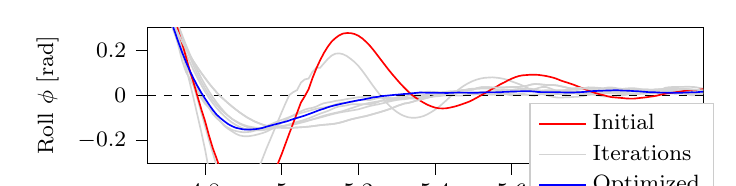
\begin{tikzpicture}[x=1in,y=1in]
  \useasboundingbox (-0.6, 0) rectangle (2.8, -0.65); %

\definecolor{darkgray176}{RGB}{176,176,176}
\definecolor{lightgray}{RGB}{211,211,211}
\definecolor{lightgray204}{RGB}{204,204,204}

\begin{axis}[
    anchor=north west,
    width=3.4in,
    height=1.3in,
    legend cell align={left},
    legend style={
      fill opacity=1,
      draw opacity=1,
      text opacity=1,
      at={(1.02,-0.32)},
      anchor=south east,
      font=\footnotesize,
      draw=lightgray204
    },
    tick align=outside,
    tick pos=left,
    x grid style={darkgray176},
    xlabel={Time [s]},
    xmin=4.65, xmax=6.1,
    xlabel shift=-1mm,
    xtick style={color=black},
    y grid style={darkgray176},
    ylabel={Roll $\phi$ [rad]},
    ymin=-0.3, ymax=0.3,
    ytick style={color=black},
    tick label style={font=\footnotesize}, %
    label style={font=\footnotesize}, %
    ]
\addplot [semithick, lightgray, forget plot]
table {%
4.00001 0.954919
4.01001 0.953935
4.02001 0.950519
4.03001 0.948766
4.04001 0.950751
4.05001 0.951926
4.06001 0.950733
4.07001 0.950185
4.08001 0.948311
4.09001 0.945215
4.10001 0.942845
4.11001 0.942911
4.12001 0.942192
4.13001 0.941415
4.14001 0.942678
4.15001 0.943144
4.16001 0.941618
4.17001 0.940693
4.18001 0.941317
4.19001 0.940513
4.20001 0.939397
4.21001 0.94034
4.22001 0.939784
4.23001 0.937579
4.24001 0.938575
4.25001 0.941119
4.26001 0.941792
4.27001 0.943734
4.28001 0.947264
4.29001 0.951157
4.30001 0.951963
4.31001 0.95316
4.32001 0.954357
4.33001 0.953032
4.34001 0.951933
4.35001 0.952564
4.36001 0.950666
4.37001 0.949786
4.38001 0.948469
4.39001 0.944855
4.40001 0.943546
4.41001 0.944058
4.42001 0.942023
4.43001 0.940797
4.44001 0.939014
4.45001 0.935831
4.46001 0.933609
4.47001 0.932402
4.48001 0.930986
4.49001 0.92996
4.50001 0.928852
4.51001 0.925983
4.52001 0.920539
4.53001 0.913789
4.54001 0.90555
4.55001 0.895133
4.56001 0.881488
4.57001 0.865807
4.58001 0.84565
4.59001 0.824403
4.60001 0.801964
4.61001 0.777846
4.62001 0.750364
4.63001 0.72076
4.64001 0.689933
4.65001 0.657808
4.66001 0.623254
4.67001 0.5825
4.68002 0.538447
4.69001 0.491941
4.70001 0.436963
4.71001 0.374683
4.72001 0.317756
4.73001 0.257473
4.74001 0.194368
4.75001 0.123951
4.76001 0.0557564
4.77001 -0.0145664
4.78001 -0.0889201
4.79001 -0.162805
4.80001 -0.241241
4.81001 -0.332329
4.82002 -0.4309
4.83001 -0.541051
4.84001 -0.60457
4.85001 -0.589754
4.86001 -0.571069
4.87001 -0.700555
4.88001 -0.810683
4.89001 -0.865681
};
\addplot [semithick, lightgray, forget plot]
table {%
4.00001 0.955874
4.01001 0.957173
4.02001 0.95416
4.03001 0.953441
4.04001 0.953806
4.05001 0.949596
4.06001 0.943598
4.07001 0.943399
4.08001 0.941089
4.09001 0.935843
4.10001 0.933637
4.11002 0.931216
4.12001 0.929857
4.13001 0.931026
4.14001 0.933612
4.15001 0.93307
4.16001 0.933727
4.17001 0.937497
4.18001 0.936933
4.19001 0.936608
4.20001 0.939915
4.21002 0.940431
4.22001 0.941085
4.23001 0.944354
4.24001 0.947742
4.25001 0.947612
4.26001 0.946556
4.27001 0.950523
4.28001 0.951139
4.29001 0.947662
4.30001 0.951149
4.31001 0.9511
4.32001 0.947474
4.33001 0.946316
4.34001 0.943545
4.35001 0.940297
4.36001 0.940332
4.37001 0.939822
4.38001 0.939224
4.39001 0.943343
4.40001 0.949233
4.41001 0.949774
4.42001 0.948405
4.43001 0.950953
4.44001 0.947397
4.45001 0.944707
4.46001 0.945336
4.47001 0.945872
4.48001 0.941561
4.49001 0.935867
4.50001 0.928405
4.51001 0.919408
4.52001 0.909898
4.53001 0.900033
4.54001 0.889089
4.55001 0.878367
4.56001 0.866737
4.57001 0.850663
4.58001 0.833782
4.59001 0.816707
4.60002 0.795381
4.61001 0.770038
4.62002 0.741737
4.63001 0.710654
4.64001 0.677006
4.65001 0.64046
4.66001 0.601212
4.67001 0.560703
4.68001 0.517935
4.69001 0.467806
4.70001 0.409487
4.71001 0.349899
4.72001 0.287928
4.73001 0.220779
4.74001 0.152827
4.75001 0.103571
4.76001 0.0747054
4.77001 0.0411095
4.78001 -0.0155789
4.79001 -0.0768556
4.80001 -0.136687
4.81001 -0.198649
4.82001 -0.254888
4.83001 -0.312969
4.84001 -0.367689
4.85001 -0.407885
4.86001 -0.436372
4.87001 -0.455743
4.88002 -0.46507
4.89001 -0.464822
4.90001 -0.457726
4.91001 -0.441574
4.92002 -0.399964
4.93001 -0.35441
4.94001 -0.322248
4.95001 -0.279119
4.96001 -0.235467
4.97001 -0.195315
4.98001 -0.154834
4.99001 -0.114139
5.00001 -0.0739386
5.01001 -0.0344116
5.02001 0.0023271
5.03001 0.0145526
5.04001 0.0235644
5.05001 0.0566951
5.06001 0.070861
5.07001 0.0745125
5.08001 0.104499
5.09001 0.12156
5.10001 0.122173
5.11001 0.141751
5.12002 0.160942
5.13001 0.176235
5.14001 0.18462
5.15001 0.186287
5.16001 0.182423
5.17001 0.174023
5.18001 0.161784
5.19001 0.147982
5.20001 0.1306
5.21001 0.109645
5.22001 0.0864509
5.23001 0.0622249
5.24001 0.0384929
5.25001 0.0161677
5.26001 -0.00530279
5.27001 -0.0255307
5.28001 -0.0438854
5.29001 -0.0596132
5.30001 -0.0728233
5.31001 -0.0836398
5.32001 -0.0915164
5.33001 -0.0968035
5.34001 -0.09914
5.35001 -0.0987996
5.36001 -0.0962236
5.37001 -0.0915099
5.38002 -0.0839064
5.39001 -0.0741699
5.40002 -0.0635139
5.41001 -0.0510597
5.42001 -0.036469
5.43001 -0.0213037
5.44001 -0.00555365
5.45001 0.00948541
5.46001 0.0237127
5.47001 0.0365845
5.48001 0.0475384
5.49001 0.0568116
5.50001 0.0647128
5.51001 0.0705711
5.52001 0.0751396
5.53001 0.0779092
5.54001 0.0791338
5.55001 0.0800839
5.56001 0.0785399
5.57001 0.0764879
5.58001 0.0731311
5.59001 0.0685324
5.60001 0.0618979
5.61001 0.0559079
5.62001 0.0496674
5.63001 0.0424562
5.64001 0.0339704
5.65001 0.0260431
5.66001 0.0192902
5.67001 0.0128377
5.68001 0.00690154
5.69001 0.00173189
5.70001 -0.0034601
5.71001 -0.0073229
5.72001 -0.00960177
5.73001 -0.00988567
5.74001 -0.00836379
5.75002 -0.0083094
5.76001 -0.00686752
5.77001 -0.00623535
5.78001 -0.00461075
5.79001 -0.00181557
5.80001 0.00231593
5.81001 0.0051281
5.82001 0.0090324
5.83001 0.012415
5.84001 0.0146892
5.85001 0.0170136
5.86001 0.0208212
5.87001 0.0227832
5.88001 0.0249049
5.89001 0.0253654
5.90001 0.0259631
5.91001 0.0254183
5.92001 0.0265644
5.93001 0.026186
5.94001 0.023985
5.95001 0.023199
5.96001 0.0230142
5.97001 0.0244422
5.98001 0.0256234
5.99001 0.0255763
6.00001 0.0236127
6.01001 0.0253032
6.02001 0.0271641
6.03001 0.0282546
6.04001 0.0303159
6.05001 0.0291287
6.06001 0.0266044
6.07001 0.0260709
6.08001 0.0251851
6.09001 0.0239004
6.10002 0.0243138
6.11001 0.0237204
6.12001 0.0192926
6.13001 0.0133656
6.14001 0.0101238
6.15001 0.00588845
6.16001 0.00149898
6.17001 -0.00161552
6.18001 -0.00544931
6.19001 -0.00704257
6.20001 -0.00781557
6.21001 -0.00823132
6.22001 -0.00774279
6.23001 -0.00651008
6.24001 -0.00545845
6.25002 -0.00217255
6.26001 0.00160714
6.27001 0.00634357
6.28001 0.0108101
6.29001 0.0141289
6.30001 0.0170369
6.31001 0.0200054
6.32001 0.0230405
6.33001 0.0254658
6.34001 0.0271504
6.35001 0.0293872
6.36001 0.0319282
6.37001 0.0333152
6.38001 0.0327345
6.39001 0.0331309
6.40001 0.03421
6.41001 0.0327941
6.42001 0.0336363
6.43001 0.0343782
6.44001 0.034419
6.45001 0.0337271
6.46001 0.0309791
6.47001 0.0284145
6.48001 0.0270752
6.49001 0.0261552
6.50001 0.0256569
6.51001 0.0247457
6.52001 0.0236982
6.53001 0.0225476
6.54001 0.0203995
6.55001 0.0177654
6.56001 0.0157924
6.57001 0.0134728
6.58001 0.0118333
6.59002 0.0109949
6.60001 0.00997985
6.61001 0.00948895
6.62001 0.00952847
6.63001 0.0100599
6.64001 0.0114475
6.65001 0.013067
6.66001 0.0151015
6.67001 0.016869
6.68001 0.0181008
6.69001 0.0175328
6.70001 0.0168946
6.71001 0.0170586
6.72001 0.0180805
6.73001 0.017693
6.74001 0.0181836
6.75001 0.0190716
6.76001 0.019448
6.77001 0.0207196
6.78001 0.0212237
6.79001 0.0224218
6.80001 0.0234507
6.81001 0.0235475
6.82001 0.0236325
6.83001 0.0248464
6.84001 0.0253856
6.85001 0.0246406
6.86001 0.0245321
6.87001 0.0245615
6.88001 0.0243855
6.89001 0.0250201
6.90001 0.0253758
6.91001 0.0249001
6.92001 0.0241795
6.93001 0.0232142
6.94001 0.0218572
6.95001 0.0201065
6.96001 0.0193738
6.97001 0.0175293
6.98001 0.015078
6.99001 0.0128541
7.00001 0.0111509
7.01001 0.00957813
7.02001 0.00860484
7.03001 0.00871554
7.04001 0.00924735
7.05001 0.00885662
7.06001 0.00850326
7.07001 0.00718396
7.08001 0.00519483
7.09001 0.00465297
7.10001 0.00448709
7.11001 0.00574355
7.12001 0.00868301
7.13001 0.012375
7.14001 0.0161414
7.15001 0.0196374
7.16001 0.0216763
7.17001 0.0223969
7.18001 0.0225917
7.19001 0.0233887
7.20001 0.0236848
7.21001 0.0248765
7.22001 0.0253656
7.23001 0.025692
7.24001 0.0248644
7.25001 0.0229731
7.26001 0.0207655
7.27001 0.0193572
7.28001 0.0183324
7.29001 0.0176309
7.30001 0.0175105
7.31001 0.0159523
7.32001 0.0144077
7.33001 0.0134611
7.34001 0.0128376
7.35001 0.0145073
7.36001 0.0166927
7.37001 0.0170418
7.38001 0.0165109
7.39001 0.0166628
7.40001 0.0165321
7.41001 0.0163708
7.42002 0.0162392
7.43001 0.0154787
7.44001 0.0140755
7.45001 0.0136058
7.46001 0.0133357
7.47001 0.0138056
7.48001 0.0151139
7.49001 0.015419
};
\addplot [semithick, lightgray, forget plot]
table {%
4.00001 0.972877
4.01001 0.973731
4.02001 0.972592
4.03001 0.973954
4.04001 0.972979
4.05001 0.970286
4.06001 0.969284
4.07001 0.968957
4.08001 0.966313
4.09001 0.9668
4.10001 0.967188
4.11001 0.965776
4.12001 0.965822
4.13001 0.965479
4.14001 0.961261
4.15001 0.957719
4.16001 0.956109
4.17002 0.951114
4.18001 0.948019
4.19001 0.948968
4.20001 0.949316
4.21001 0.949495
4.22001 0.949684
4.23001 0.949036
4.24001 0.947851
4.25001 0.951634
4.26001 0.953557
4.27001 0.954483
4.28001 0.955768
4.29001 0.955646
4.30001 0.955127
4.31001 0.955423
4.32001 0.9536
4.33001 0.952275
4.34001 0.952753
4.35001 0.951744
4.36001 0.951569
4.37001 0.954217
4.38001 0.953989
4.39001 0.955284
4.40001 0.956728
4.41001 0.955403
4.42001 0.955174
4.43001 0.952189
4.44001 0.958554
4.45001 0.960198
4.46001 0.960377
4.47001 0.961496
4.48001 0.961152
4.49001 0.959871
4.50001 0.957134
4.51001 0.953922
4.52001 0.949237
4.53001 0.942699
4.54002 0.933195
4.55001 0.920498
4.56001 0.904919
4.57001 0.887653
4.58001 0.869425
4.59001 0.849223
4.60001 0.827876
4.61001 0.803056
4.62001 0.776937
4.63001 0.748503
4.64001 0.715993
4.65001 0.680609
4.66001 0.64007
4.67001 0.594391
4.68001 0.547198
4.69001 0.500537
4.70001 0.452827
4.71001 0.404382
4.72001 0.357367
4.73001 0.311143
4.74001 0.266499
4.75001 0.223077
4.76001 0.18282
4.77001 0.145377
4.78001 0.109963
4.79001 0.0766149
4.80001 0.0460812
4.81001 0.0179911
4.82001 -0.00780249
4.83001 -0.0315204
4.84001 -0.052856
4.85001 -0.0726176
4.86001 -0.0895991
4.87001 -0.104037
4.88001 -0.1155
4.89001 -0.125829
4.90001 -0.133729
4.91001 -0.13994
4.92001 -0.14468
4.93001 -0.147446
4.94001 -0.148842
4.95001 -0.148305
4.96001 -0.146326
4.97001 -0.144101
4.98001 -0.141438
4.99001 -0.138315
5.00001 -0.135526
5.01001 -0.133787
5.02001 -0.13159
5.03001 -0.128889
5.04001 -0.125504
5.05001 -0.121193
5.06001 -0.116947
5.07001 -0.111851
5.08001 -0.106521
5.09001 -0.100633
5.10001 -0.095128
5.11001 -0.0898115
5.12001 -0.0853031
5.13001 -0.080788
5.14001 -0.0772907
5.15001 -0.0732643
5.16001 -0.0689704
5.17001 -0.0631665
5.18001 -0.0574755
5.19001 -0.0519396
5.20001 -0.0463198
5.21001 -0.0409878
5.22001 -0.0364573
5.23002 -0.0326291
5.24001 -0.0298216
5.25001 -0.026596
5.26002 -0.0245104
5.27001 -0.0231646
5.28001 -0.0211835
5.29001 -0.0185091
5.30001 -0.0138798
5.31001 -0.00912922
5.32001 -0.00520699
5.33001 -0.00180248
5.34001 0.000307473
5.35001 0.000543231
5.36001 0.000447465
5.37001 0.00170623
5.38001 0.00192465
5.39001 0.00270124
5.40001 0.00314686
5.41001 0.00440092
5.42001 0.00729108
5.43001 0.00893674
5.44001 0.00978461
5.45001 0.00967891
5.46002 0.00934481
5.47001 0.0103039
5.48001 0.0114628
5.49001 0.0115211
5.50001 0.0124449
5.51001 0.0132091
5.52001 0.0145515
5.53001 0.0155974
5.54001 0.0170559
5.55001 0.0180617
5.56001 0.0187842
5.57001 0.0157333
5.58001 0.00965324
5.59001 0.00307864
5.60001 -1.04589e-05
5.61001 0.00332827
5.62001 0.00623468
5.63001 0.00723649
5.64001 0.0039451
5.65001 0.000189248
5.66001 -0.00140704
5.67001 0.00368779
5.68001 0.00846212
5.69001 0.00961603
5.70001 0.00950646
5.71001 0.00979027
5.72001 0.0129055
5.73001 0.0204217
5.74001 0.0241903
5.75001 0.0252864
5.76001 0.0248667
5.77001 0.0241476
5.78001 0.0271491
5.79001 0.0324994
5.80001 0.0358615
5.81001 0.0353737
5.82001 0.0343839
5.83001 0.0326828
5.84001 0.0319784
5.85001 0.0346396
5.86001 0.0354741
5.87001 0.033306
5.88001 0.0287556
5.89001 0.0288937
5.90001 0.030965
5.91001 0.0318608
5.92001 0.0318218
5.93001 0.0296963
5.94001 0.0264251
5.95001 0.0214655
5.96001 0.0200725
5.97001 0.0249024
5.98001 0.0247417
5.99001 0.0212467
6.00001 0.0159614
6.01001 0.0115762
6.02001 0.0102444
6.03001 0.0107462
6.04001 0.0107714
6.05001 0.00837621
6.06001 0.00435207
6.07001 0.00031038
6.08001 0.00113518
6.09001 0.00364642
6.10001 0.00727728
6.11001 0.00685849
6.12001 0.00398574
6.13001 0.00168327
6.14002 0.0052015
6.15001 0.00866401
6.16001 0.0104066
6.17001 0.00967215
6.18001 0.00882349
6.19001 0.00747275
6.20001 0.00657166
6.21001 0.00538778
6.22002 0.00529898
6.23001 0.00480295
6.24001 0.00435672
6.25001 0.00318379
6.26001 0.00284049
6.27001 0.00305044
6.28001 0.00448139
6.29001 0.00492134
6.30001 0.00703276
6.31001 0.00828699
6.32001 0.0103116
6.33001 0.013615
6.34001 0.0154761
6.35001 0.0186655
6.36001 0.0212083
6.37001 0.0231545
6.38001 0.0230125
6.39001 0.0208168
6.40002 0.019771
6.41001 0.0198034
6.42001 0.0201105
6.43001 0.0207434
6.44001 0.0228352
6.45001 0.0242081
6.46001 0.0255973
6.47001 0.0259693
6.48001 0.0250942
6.49001 0.02508
6.50001 0.0250542
6.51001 0.0245747
6.52001 0.0250737
6.53001 0.0273858
6.54001 0.0272022
6.55001 0.0275026
6.56001 0.0273491
6.57001 0.0262149
6.58001 0.0248592
6.59001 0.0246739
6.60001 0.024405
6.61001 0.0244691
6.62001 0.0237829
6.63001 0.0213181
6.64001 0.0205333
6.65001 0.0190298
6.66001 0.0200424
6.67001 0.0194996
6.68001 0.0172704
6.69001 0.0155445
6.70001 0.0134142
6.71001 0.0117996
6.72001 0.0130572
6.73001 0.0163603
6.74001 0.0179763
6.75001 0.017514
6.76001 0.0162724
6.77001 0.0157425
6.78001 0.0172847
6.79001 0.0187147
6.80001 0.0194545
6.81001 0.0203751
6.82001 0.0194382
6.83001 0.0192013
6.84001 0.0189622
6.85001 0.0199979
6.86001 0.0199297
6.87001 0.018717
6.88001 0.0168069
6.89001 0.017366
6.90001 0.0167297
6.91001 0.0170327
6.92001 0.0157155
6.93001 0.0149145
6.94001 0.0146821
6.95001 0.0162383
6.96001 0.0193127
6.97001 0.0212287
6.98001 0.020861
6.99001 0.0193994
7.00001 0.0167875
7.01001 0.0167924
7.02002 0.0179665
7.03001 0.0172425
7.04002 0.0167472
7.05001 0.0169628
7.06001 0.0179524
7.07001 0.0184956
7.08001 0.0185696
7.09001 0.0185487
7.10001 0.0199485
7.11001 0.0215191
7.12001 0.0214788
7.13001 0.02009
7.14001 0.0182049
7.15001 0.0168345
7.16001 0.0154892
7.17001 0.0155129
7.18001 0.014566
7.19001 0.0139941
7.20001 0.0142504
7.21001 0.0135986
7.22001 0.0137709
7.23001 0.0155569
7.24001 0.0170832
7.25001 0.0168053
7.26001 0.0160929
7.27001 0.0158829
7.28001 0.0161036
7.29001 0.0156839
7.30001 0.0157255
7.31001 0.0160285
7.32001 0.0170787
7.33001 0.0166402
7.34001 0.0182554
7.35001 0.018331
7.36001 0.0184755
7.37001 0.0185963
7.38001 0.0182871
7.39001 0.018462
7.40001 0.0185368
7.41001 0.0190687
7.42001 0.0182683
7.43001 0.0170894
7.44001 0.0167427
7.45001 0.0164423
7.46001 0.0155252
7.47001 0.0138289
7.48001 0.0131732
7.49001 0.0116233
};
\addplot [semithick, lightgray, forget plot]
table {%
4.00001 0.946419
4.01001 0.949414
4.02001 0.951962
4.03001 0.955267
4.04001 0.95617
4.05001 0.957309
4.06001 0.959118
4.07001 0.95889
4.08001 0.957274
4.09002 0.956349
4.10001 0.954898
4.11001 0.954604
4.12001 0.955499
4.13001 0.955097
4.14001 0.952782
4.15001 0.95294
4.16001 0.952039
4.17001 0.952261
4.18001 0.953671
4.19001 0.952651
4.20001 0.950464
4.21001 0.949777
4.22001 0.946882
4.23001 0.94391
4.24001 0.941303
4.25001 0.937744
4.26001 0.934414
4.27001 0.933527
4.28001 0.932337
4.29001 0.933083
4.30001 0.935129
4.31001 0.935249
4.32001 0.937285
4.33001 0.939055
4.34001 0.939364
4.35001 0.940931
4.36001 0.941981
4.37001 0.941652
4.38001 0.941967
4.39001 0.942011
4.40002 0.942329
4.41001 0.94287
4.42001 0.942739
4.43001 0.941111
4.44001 0.940603
4.45001 0.939175
4.46001 0.93764
4.47001 0.935145
4.48001 0.930425
4.49001 0.924369
4.50001 0.919476
4.51001 0.913198
4.52001 0.906726
4.53001 0.899254
4.54001 0.88928
4.55001 0.877407
4.56001 0.862613
4.57001 0.844831
4.58001 0.82653
4.59001 0.806742
4.60001 0.784963
4.61001 0.758848
4.62001 0.729224
4.63002 0.698517
4.64001 0.66688
4.65001 0.629699
4.66001 0.586509
4.67001 0.54217
4.68001 0.498023
4.69001 0.453099
4.70001 0.405535
4.71001 0.360567
4.72001 0.315785
4.73001 0.270936
4.74001 0.227094
4.75001 0.185772
4.76001 0.147548
4.77001 0.111193
4.78001 0.0768419
4.79001 0.0451747
4.80001 0.0156649
4.81001 -0.0110818
4.82001 -0.0346415
4.83001 -0.0559563
4.84001 -0.0749307
4.85001 -0.0914892
4.86001 -0.106689
4.87001 -0.120016
4.88001 -0.13057
4.89001 -0.139404
4.90001 -0.146437
4.91001 -0.151028
4.92001 -0.153705
4.93001 -0.154875
4.94001 -0.154747
4.95001 -0.153993
4.96001 -0.151823
4.97001 -0.148724
4.98001 -0.145273
4.99001 -0.1417
5.00001 -0.137359
5.01001 -0.133661
5.02002 -0.129671
5.03001 -0.125079
5.04001 -0.120829
5.05001 -0.116941
5.06001 -0.113761
5.07001 -0.110252
5.08001 -0.106095
5.09001 -0.102681
5.10001 -0.0980731
5.11001 -0.0936991
5.12001 -0.0886019
5.13001 -0.0842569
5.14001 -0.0799713
5.15001 -0.0762929
5.16001 -0.0729892
5.17001 -0.070455
5.18001 -0.0674742
5.19001 -0.0646513
5.20001 -0.0615549
5.21001 -0.056765
5.22001 -0.0516172
5.23001 -0.0470935
5.24001 -0.043229
5.25001 -0.0400706
5.26001 -0.0361415
5.27001 -0.0322565
5.28001 -0.0273737
5.29001 -0.0236432
5.30001 -0.0203936
5.31001 -0.0181014
5.32001 -0.0168981
5.33001 -0.0144126
5.34001 -0.0097215
5.35001 -0.00284872
5.36001 -0.00188786
5.37001 -0.00388264
5.38001 -0.00465474
5.39001 -0.00367397
5.40001 0.00151085
5.41001 0.00667758
5.42001 0.00855511
5.43001 0.00811701
5.44001 0.00769768
5.45001 0.0102624
5.46001 0.0157383
5.47001 0.0222825
5.48001 0.0253331
5.49001 0.0288603
5.50001 0.0293773
5.51001 0.0293247
5.52001 0.0299763
5.53001 0.030486
5.54001 0.0297789
5.55001 0.0273694
5.56001 0.0245396
5.57001 0.0234423
5.58001 0.024605
5.59001 0.0254538
5.60001 0.0246505
5.61001 0.0271795
5.62001 0.0288758
5.63001 0.0298146
5.64001 0.0304664
5.65001 0.0295059
5.66001 0.0264178
5.67001 0.0227455
5.68001 0.020417
5.69001 0.0195495
5.70001 0.0201335
5.71001 0.0202447
5.72001 0.0184347
5.73001 0.0146481
5.74001 0.0116202
5.75001 0.0138581
5.76001 0.0152867
5.77001 0.0164518
5.78001 0.0154036
5.79001 0.011125
5.80001 0.00698481
5.81001 0.00603119
5.82001 0.00732198
5.83001 0.00972011
5.84001 0.010736
5.85001 0.0108218
5.86001 0.00969336
5.87001 0.00893925
5.88001 0.00693253
5.89001 0.0060886
5.90001 0.00596518
5.91001 0.00424521
5.92001 0.00398766
5.93001 0.00635564
5.94001 0.0105993
5.95001 0.013383
5.96001 0.015569
5.97001 0.0155029
5.98001 0.0158269
5.99001 0.0236469
6.00001 0.033332
6.01001 0.036218
6.02001 0.0371108
6.03001 0.0373166
6.04001 0.0377398
6.05001 0.0379009
6.06001 0.0386002
6.07001 0.0376073
6.08001 0.0366547
6.09002 0.0329998
6.10001 0.0305899
6.11001 0.0295154
6.12001 0.0287778
6.13001 0.0276964
6.14001 0.0249047
6.15001 0.026339
6.16001 0.0304012
6.17001 0.0348539
6.18001 0.0397765
6.19001 0.0414654
6.20001 0.0390074
6.21001 0.0340915
6.22001 0.0281846
6.23001 0.0251852
6.24001 0.0231075
6.25001 0.0235553
6.26001 0.0236924
6.27001 0.0225179
6.28001 0.0204476
6.29001 0.0204411
6.30001 0.0210292
6.31001 0.022517
6.32001 0.0223582
6.33001 0.0209943
6.34001 0.0205615
6.35001 0.0210105
6.36001 0.020652
6.37001 0.0212189
6.38001 0.0200609
6.39001 0.0190189
6.40001 0.0181715
6.41001 0.0174401
6.42001 0.0167211
6.43001 0.016551
6.44001 0.0164934
6.45001 0.0170906
6.46001 0.0179473
6.47002 0.0184691
6.48001 0.0200024
6.49001 0.0198402
6.50001 0.0193541
6.51001 0.0199686
6.52001 0.0204116
6.53001 0.0212379
6.54001 0.0215131
6.55001 0.0222589
6.56001 0.0224987
6.57001 0.024358
6.58001 0.0250581
6.59001 0.0267459
6.60001 0.0272654
6.61001 0.0268706
6.62001 0.0256553
6.63001 0.0244031
6.64001 0.024287
6.65001 0.0243238
6.66001 0.0256574
6.67001 0.0268259
6.68001 0.0267014
6.69001 0.0272008
6.70001 0.0277592
6.71001 0.0261576
6.72001 0.0253099
6.73001 0.0254433
6.74001 0.0254001
6.75001 0.0248796
6.76001 0.023793
6.77001 0.0240521
6.78001 0.0247568
6.79001 0.0267093
6.80001 0.0277971
6.81001 0.0277349
6.82001 0.0278811
6.83001 0.026735
6.84001 0.02588
6.85001 0.0259447
6.86001 0.0248913
6.87001 0.0240472
6.88001 0.0233357
6.89001 0.0231445
6.90001 0.0230464
6.91001 0.0229388
6.92001 0.0225566
6.93001 0.0222874
6.94001 0.0209788
6.95001 0.0205788
6.96001 0.0214717
6.97001 0.0223112
6.98001 0.0227745
6.99001 0.022172
7.00001 0.0220413
7.01001 0.0206335
7.02001 0.0208009
7.03001 0.0202277
7.04001 0.0185459
7.05001 0.0183632
7.06001 0.0179554
7.07001 0.0177269
7.08001 0.0185123
7.09001 0.0174033
7.10001 0.0168893
7.11001 0.0153882
7.12001 0.0145074
7.13001 0.0137256
7.14001 0.0134562
7.15001 0.0138745
7.16001 0.014198
7.17001 0.0125371
7.18001 0.0112309
7.19001 0.0112183
7.20001 0.00827275
7.21001 0.00625936
7.22001 0.00462928
7.23001 0.00366348
7.24001 0.00377415
7.25001 0.00399537
7.26001 0.00625727
7.27001 0.00751967
7.28001 0.00826801
7.29001 0.00643053
7.30001 0.00620676
7.31001 0.00637594
7.32001 0.00763974
7.33001 0.00756693
7.34001 0.00682158
7.35001 0.00166627
7.36001 -0.00249879
7.37001 -0.00445626
7.38001 -0.00501977
7.39001 -0.00515182
7.40001 -0.00224122
7.41001 -0.00204821
7.42001 -0.00151119
7.43001 0.00094121
7.44001 0.00655039
7.45001 0.00954279
7.46001 0.0110264
7.47001 0.010725
7.48001 0.0127952
7.49001 0.0148989
};
\addplot [semithick, lightgray, forget plot]
table {%
4.00001 0.95331
4.01001 0.951401
4.02001 0.951952
4.03001 0.95188
4.04001 0.951509
4.05001 0.952011
4.06001 0.951617
4.07001 0.95006
4.08001 0.950107
4.09001 0.949885
4.10001 0.94915
4.11001 0.950455
4.12001 0.950412
4.13001 0.94996
4.14001 0.951057
4.15001 0.949824
4.16001 0.951628
4.17001 0.954116
4.18001 0.953154
4.19002 0.954214
4.20001 0.953552
4.21001 0.952199
4.22001 0.954159
4.23001 0.954436
4.24001 0.953748
4.25001 0.955699
4.26001 0.955118
4.27001 0.954601
4.28001 0.95395
4.29001 0.95318
4.30001 0.953669
4.31001 0.954428
4.32001 0.953149
4.33001 0.951957
4.34001 0.951956
4.35001 0.950221
4.36001 0.950751
4.37001 0.950572
4.38001 0.949471
4.39001 0.949033
4.40001 0.94632
4.41001 0.945209
4.42001 0.945952
4.43001 0.940726
4.44001 0.935563
4.45001 0.932154
4.46001 0.92857
4.47001 0.926928
4.48001 0.92511
4.49001 0.92272
4.50001 0.918467
4.51001 0.912851
4.52001 0.906295
4.53001 0.898033
4.54001 0.887991
4.55001 0.876056
4.56001 0.862685
4.57002 0.85034
4.58001 0.836722
4.59001 0.820541
4.60001 0.801625
4.61001 0.78004
4.62001 0.754724
4.63001 0.726631
4.64001 0.693896
4.65001 0.660597
4.66001 0.621135
4.67001 0.578072
4.68001 0.53347
4.69001 0.52707
4.70001 0.48069
4.71001 0.408569
4.72001 0.358278
4.73001 0.30816
4.74001 0.258544
4.75001 0.213306
4.76001 0.170169
4.77001 0.130616
4.78002 0.0933092
4.79001 0.0600447
4.80001 0.0299587
4.81001 0.00273493
4.82001 -0.0217778
4.83001 -0.0426939
4.84001 -0.060949
4.85001 -0.0769118
4.86001 -0.0905433
4.87001 -0.103688
4.88001 -0.11374
4.89002 -0.123047
4.90001 -0.13024
4.91001 -0.135921
4.92001 -0.139588
4.93001 -0.142422
4.94001 -0.144157
4.95001 -0.146253
4.96001 -0.146525
4.97001 -0.14612
4.98001 -0.143238
4.99001 -0.140573
5.00001 -0.137674
5.01001 -0.133287
5.02001 -0.127848
5.03001 -0.122709
5.04001 -0.117381
5.05001 -0.112894
5.06001 -0.107469
5.07001 -0.101398
5.08001 -0.0951407
5.09001 -0.0877634
5.10001 -0.0809552
5.11001 -0.0752709
5.12001 -0.0690532
5.13001 -0.0616177
5.14001 -0.0538619
5.15001 -0.0489662
5.16002 -0.0465956
5.17001 -0.0441008
5.18001 -0.0397559
5.19001 -0.0389004
5.20001 -0.0392375
5.21001 -0.0391223
5.22001 -0.0393304
5.23001 -0.0388662
5.24001 -0.0360773
5.25001 -0.0308164
5.26001 -0.022261
5.27001 -0.0212304
5.28001 -0.0195365
5.29001 -0.0142924
5.30002 -0.00870108
5.31001 -0.00194798
5.32001 0.00461612
5.33001 0.00787879
5.34001 0.00872043
5.35001 0.00918523
5.36001 0.0119437
5.37001 0.0139953
5.38001 0.0163535
5.39001 0.0158325
5.40001 0.0147314
5.41001 0.0142157
5.42001 0.0146604
5.43001 0.015982
5.44001 0.0183134
5.45001 0.0173605
5.46001 0.0153753
5.47001 0.0139152
5.48001 0.0131596
5.49001 0.0120897
5.50001 0.0113569
5.51001 0.0100465
5.52001 0.00755721
5.53001 0.00460454
5.54001 0.00383131
5.55001 0.00410933
5.56001 0.00565571
5.57001 0.00656967
5.58001 0.007451
5.59001 0.00779631
5.60001 0.0119774
5.61001 0.017357
5.62001 0.0195544
5.63001 0.0206251
5.64001 0.0194799
5.65001 0.0173929
5.66001 0.0186137
5.67001 0.0212754
5.68001 0.0213761
5.69001 0.0234184
5.70001 0.0226412
5.71001 0.0211219
5.72001 0.0225768
5.73001 0.0226602
5.74001 0.0228247
5.75001 0.0201739
5.76001 0.0165518
5.77001 0.0164319
5.78001 0.0165179
5.79001 0.0163243
5.80001 0.0154135
5.81001 0.015585
5.82001 0.0134326
5.83001 0.0119781
5.84001 0.0136505
5.85001 0.014965
5.86001 0.0181047
5.87001 0.0177852
5.88001 0.0154472
5.89001 0.0151608
5.90001 0.0155683
5.91001 0.0176459
5.92001 0.0196816
5.93002 0.0207862
5.94001 0.0187752
5.95001 0.018635
5.96001 0.019523
5.97001 0.0209211
5.98001 0.0217617
5.99001 0.0224011
6.00001 0.0225844
6.01001 0.0198021
6.02001 0.0203493
6.03001 0.020761
6.04001 0.0208647
6.05001 0.0207945
6.06001 0.0184302
6.07001 0.01663
6.08001 0.0168274
6.09001 0.0162265
6.10001 0.0174185
6.11002 0.0179812
6.12001 0.0152079
6.13001 0.0101558
6.14001 0.0108419
6.15001 0.0116576
6.16001 0.0128171
6.17001 0.0128861
6.18001 0.0102696
6.19001 0.00774918
6.20001 0.0082697
6.21001 0.00998461
6.22001 0.0116243
6.23002 0.0117109
6.24001 0.0120411
6.25002 0.0121135
6.26001 0.0141222
6.27001 0.0174458
6.28001 0.020597
6.29001 0.0203372
6.30001 0.0157084
6.31001 0.0116182
6.32001 0.00991456
6.33001 0.00913431
6.34001 0.00995956
6.35001 0.0103921
6.36001 0.0096199
6.37001 0.00803361
6.38001 0.0079392
6.39001 0.00877574
6.40001 0.00960841
6.41001 0.0106979
6.42001 0.0108407
6.43001 0.0103643
6.44001 0.0128697
6.45001 0.0167146
6.46001 0.0209862
6.47001 0.023874
6.48001 0.0256323
6.49001 0.0266592
6.50001 0.0267481
6.51001 0.0279881
6.52001 0.0287243
6.53001 0.0278185
6.54001 0.0247951
6.55002 0.0229037
6.56001 0.0232192
6.57001 0.024258
6.58001 0.0252279
6.59001 0.0236992
6.60001 0.0213202
6.61001 0.0209308
6.62001 0.0211255
6.63001 0.0218541
6.64001 0.0217873
6.65001 0.0211447
6.66001 0.0203414
6.67001 0.0208489
6.68001 0.0209263
6.69001 0.0221029
6.70001 0.0229623
6.71001 0.0220226
6.72001 0.0211365
6.73001 0.0206089
6.74001 0.0195129
6.75001 0.0179487
6.76001 0.0176838
6.77001 0.0176622
6.78001 0.018655
6.79001 0.0193092
6.80001 0.0200549
6.81001 0.0204278
6.82001 0.0203598
6.83001 0.0209536
6.84001 0.0205623
6.85001 0.0198917
6.86001 0.0199374
6.87001 0.0200216
6.88001 0.0188174
6.89001 0.0191868
6.90001 0.0189662
6.91001 0.0186873
6.92001 0.0190116
6.93001 0.019299
6.94001 0.0206718
6.95001 0.0200036
6.96001 0.0189271
6.97001 0.0190353
6.98002 0.0177104
6.99001 0.0158606
7.00001 0.0165931
7.01001 0.0158142
7.02001 0.0146992
7.03001 0.0153864
7.04001 0.0144045
7.05001 0.0140768
7.06002 0.0142533
7.07001 0.0142801
7.08001 0.0167277
7.09001 0.0173127
7.10001 0.0191686
7.11001 0.01891
7.12001 0.0192387
7.13001 0.0198096
7.14001 0.0187582
7.15001 0.017317
7.16001 0.0167591
7.17001 0.0165128
7.18001 0.0153664
7.19001 0.0154068
7.20001 0.014599
7.21001 0.0128159
7.22001 0.0138268
7.23001 0.0133785
7.24002 0.0131143
7.25002 0.0128441
7.26002 0.0130747
7.27001 0.0135959
7.28001 0.0132997
7.29001 0.0126938
7.30001 0.0105571
7.31001 0.00958063
7.32001 0.008515
7.33001 0.00825546
7.34001 0.00744121
7.35001 0.00734552
7.36001 0.00564966
7.37001 0.00478597
7.38001 0.00443632
7.39001 0.0049641
7.40001 0.00729201
7.41001 0.00838708
7.42001 0.0112425
7.43001 0.0158789
7.44001 0.0185929
7.45001 0.0215484
7.46001 0.0233908
7.47001 0.0240931
7.48001 0.0235208
7.49001 0.0245903
};
\addplot [semithick, lightgray, forget plot]
table {%
4.00001 0.948322
4.01001 0.948594
4.02001 0.949613
4.03001 0.949013
4.04001 0.948075
4.05001 0.950124
4.06001 0.949238
4.07001 0.948515
4.08001 0.949176
4.09001 0.946518
4.10001 0.945398
4.11002 0.943218
4.12001 0.94176
4.13001 0.941617
4.14001 0.940667
4.15001 0.94135
4.16001 0.939329
4.17001 0.938208
4.18001 0.939851
4.19001 0.940552
4.20001 0.94435
4.21001 0.946631
4.22001 0.949192
4.23001 0.950065
4.24002 0.947995
4.25002 0.950352
4.26002 0.950472
4.27001 0.950589
4.28001 0.949426
4.29001 0.949646
4.30001 0.952143
4.31001 0.951449
4.32001 0.95082
4.33001 0.950317
4.34001 0.949677
4.35001 0.951722
4.36001 0.952704
4.37001 0.953507
4.38002 0.953144
4.39001 0.952054
4.40001 0.951434
4.41001 0.949563
4.42001 0.950321
4.43001 0.960424
4.44001 0.967962
4.45001 0.972445
4.46001 0.973349
4.47001 0.973845
4.48001 0.97196
4.49001 0.967939
4.50001 0.960865
4.51001 0.951472
4.52001 0.94063
4.53001 0.929702
4.54001 0.919036
4.55001 0.905856
4.56001 0.888571
4.57001 0.870617
4.58001 0.84983
4.59001 0.828037
4.60001 0.801689
4.61001 0.771998
4.62001 0.740726
4.63001 0.707468
4.64001 0.672023
4.65001 0.636581
4.66001 0.596175
4.67002 0.552978
4.68001 0.507604
4.69001 0.46114
4.70001 0.411364
4.71001 0.360006
4.72002 0.308525
4.73001 0.255243
4.74001 0.202633
4.75001 0.152529
4.76001 0.106083
4.77001 0.0621151
4.78001 0.0227294
4.79001 -0.0130662
4.80001 -0.0378042
4.81001 -0.0535522
4.82001 -0.0822531
4.83001 -0.100937
4.84001 -0.114468
4.85001 -0.135094
4.86001 -0.148229
4.87001 -0.158907
4.88001 -0.169787
4.89001 -0.177277
4.90001 -0.180499
4.91001 -0.181202
4.92001 -0.179227
4.93001 -0.175878
4.94001 -0.171591
4.95001 -0.166772
4.96001 -0.160549
4.97001 -0.152147
4.98001 -0.142222
4.99001 -0.131583
5.00001 -0.121004
5.01001 -0.108956
5.02001 -0.0974187
5.03001 -0.0882307
5.04001 -0.0791671
5.05001 -0.0704414
5.06001 -0.0630462
5.07001 -0.0582796
5.08001 -0.0550766
5.09001 -0.0495168
5.10001 -0.0411389
5.11001 -0.0345775
5.12001 -0.0314261
5.13001 -0.0286715
5.14001 -0.0245256
5.15001 -0.0223789
5.16001 -0.0195471
5.17001 -0.0161967
5.18001 -0.0135792
5.19001 -0.0105414
5.20001 -0.00795287
5.21001 -0.00726351
5.22001 -0.00531927
5.23001 -0.0032209
5.24001 -0.00468345
5.25001 -0.00786884
5.26001 -0.0104479
5.27001 -0.0119274
5.28001 -0.013595
5.29001 -0.0126303
5.30002 -0.0120276
5.31001 -0.0130086
5.32001 -0.0119463
5.33001 -0.0111985
5.34001 -0.00920255
5.35001 -0.00772103
5.36001 -0.00789454
5.37001 -0.00827975
5.38001 -0.00847819
5.39001 -0.00508944
5.40001 -0.00124869
5.41001 0.0028599
5.42001 0.00547823
5.43001 0.00572669
5.44001 0.00654683
5.45001 0.00664459
5.46001 0.00990302
5.47001 0.0126887
5.48001 0.0107018
5.49001 0.00747047
5.50001 0.00378843
5.51001 0.00612952
5.52001 0.00576277
5.53001 0.00717602
5.54001 0.00514248
5.55001 0.00368232
5.56001 0.00273192
5.57001 0.00363234
5.58001 0.00483063
5.59001 0.00577639
5.60001 0.00558787
5.61001 0.00447062
5.62001 0.00256524
5.63001 0.00233102
5.64001 0.00271848
5.65001 0.00330483
5.66001 0.00407322
5.67001 0.00412672
5.68001 0.00467703
5.69001 0.00393994
5.70001 0.00480872
5.71001 0.00500651
5.72002 0.00607181
5.73001 0.00534215
5.74001 0.00576804
5.75001 0.00744798
5.76001 0.0095262
5.77001 0.0111391
5.78001 0.0118111
5.79001 0.0106819
5.80001 0.00958354
5.81001 0.0104635
5.82001 0.0138303
5.83001 0.0163693
5.84001 0.0167969
5.85001 0.0156951
5.86001 0.0138733
5.87001 0.0128261
5.88001 0.0134049
5.89001 0.0137005
5.90001 0.0116186
5.91001 0.0085596
5.92001 0.00634972
5.93001 0.00627609
5.94001 0.00801566
5.95001 0.0113616
5.96001 0.01107
5.97001 0.00958544
5.98001 0.00792098
5.99001 0.00879715
6.00001 0.0117636
6.01001 0.0137514
6.02001 0.0126654
6.03001 0.0108008
6.04001 0.00907165
6.05001 0.0105174
6.06001 0.0146995
6.07001 0.0178304
6.08001 0.0173674
6.09001 0.0134678
6.10001 0.010875
6.11001 0.00929226
6.12001 0.00674904
6.13001 0.00523044
6.14001 0.00390662
6.15001 0.00338741
6.16001 0.00404642
6.17001 0.00405321
6.18001 0.00497488
6.19001 0.00705311
6.20001 0.01024
6.21002 0.0127048
6.22002 0.0145753
6.23002 0.0148576
6.24002 0.0156169
6.25001 0.0154344
6.26001 0.0164583
6.27001 0.0156754
6.28001 0.0158778
6.29001 0.0170345
6.30001 0.0192059
6.31001 0.0206559
6.32001 0.019802
6.33002 0.0183944
6.34001 0.0182618
6.35001 0.0183292
6.36001 0.0185383
6.37001 0.0187158
6.38001 0.0177572
6.39001 0.0180667
6.40001 0.0178449
6.41001 0.0172054
6.42001 0.0179544
6.43001 0.0187354
6.44001 0.019239
6.45001 0.0191078
6.46001 0.0194831
6.47001 0.0198961
6.48001 0.0204233
6.49001 0.0209614
6.50001 0.0204657
6.51001 0.0191806
6.52001 0.01757
6.53001 0.0177017
6.54001 0.0180074
6.55001 0.0179469
6.56001 0.0170928
6.57001 0.0172598
6.58001 0.0166984
6.59001 0.015667
6.60001 0.0145786
6.61001 0.0125864
6.62001 0.012039
6.63001 0.0122954
6.64001 0.0135367
6.65001 0.0142078
6.66001 0.0156759
6.67001 0.0157874
6.68001 0.0163671
6.69001 0.0175241
6.70001 0.0169753
6.71001 0.0170813
6.72001 0.015292
6.73001 0.0144196
6.74001 0.0137022
6.75001 0.0120065
6.76001 0.0101986
6.77001 0.0103474
6.78001 0.00969828
6.79001 0.0103579
6.80001 0.0109971
6.81001 0.0135902
6.82001 0.0160615
6.83001 0.0182059
6.84001 0.0197977
6.85001 0.0205983
6.86001 0.0198915
6.87001 0.0187013
6.88002 0.0173759
6.89002 0.0166346
6.90001 0.0149444
6.91001 0.0152175
6.92001 0.0161604
6.93001 0.0162088
6.94001 0.0170815
6.95001 0.0189016
6.96001 0.020004
6.97001 0.0217297
6.98001 0.0224412
6.99001 0.0233735
7.00001 0.0236242
7.01001 0.0242047
7.02001 0.024801
7.03001 0.0250627
7.04001 0.0237923
7.05001 0.022058
7.06001 0.021745
7.07001 0.0204103
7.08001 0.0196197
7.09001 0.0184111
7.10001 0.0180874
7.11001 0.0195095
7.12002 0.0206662
7.13001 0.0198413
7.14001 0.0184773
7.15001 0.0154906
7.16001 0.0148547
7.17001 0.0131127
7.18001 0.0114509
7.19001 0.0105582
7.20001 0.00932709
7.21001 0.00780823
7.22001 0.00739359
7.23001 0.00708739
7.24001 0.00703212
7.25001 0.00797332
7.26001 0.00925379
7.27001 0.00991366
7.28001 0.011513
7.29001 0.0123971
7.30001 0.0126904
7.31001 0.0117101
7.32001 0.0102059
7.33001 0.0097864
7.34001 0.01121
7.35001 0.0128002
7.36002 0.0139432
7.37001 0.0139825
7.38001 0.011782
7.39001 0.00921425
7.40001 0.00776918
7.41001 0.00715558
7.42001 0.00737526
7.43001 0.0060307
7.44001 0.00529171
7.45001 0.00382934
7.46001 0.00528546
7.47001 0.00723518
7.48001 0.00878311
7.49001 0.00909896
};
\addplot [semithick, lightgray, forget plot]
table {%
4.00001 0.951297
4.01001 0.951516
4.02001 0.95277
4.03001 0.954593
4.04001 0.956476
4.05001 0.957648
4.06001 0.959493
4.07001 0.961515
4.08001 0.96101
4.09001 0.959377
4.10001 0.960373
4.11001 0.959908
4.12001 0.960863
4.13001 0.961365
4.14001 0.960265
4.15001 0.958641
4.16001 0.95462
4.17001 0.953273
4.18001 0.952414
4.19001 0.951985
4.20001 0.951106
4.21001 0.949924
4.22001 0.951469
4.23001 0.950828
4.24001 0.949878
4.25001 0.94908
4.26001 0.947459
4.27001 0.948283
4.28001 0.948336
4.29001 0.949282
4.30001 0.948897
4.31001 0.94825
4.32001 0.948494
4.33001 0.947144
4.34001 0.947268
4.35001 0.946972
4.36002 0.945867
4.37001 0.94622
4.38001 0.944021
4.39001 0.943286
4.40001 0.941172
4.41001 0.940093
4.42001 0.938827
4.43001 0.937222
4.44001 0.935531
4.45001 0.933448
4.46001 0.93369
4.47001 0.934532
4.48001 0.934623
4.49001 0.932972
4.50001 0.929463
4.51001 0.923816
4.52001 0.915646
4.53001 0.906076
4.54001 0.896178
4.55001 0.883698
4.56001 0.866485
4.57001 0.846923
4.58001 0.827253
4.59001 0.805131
4.60001 0.780449
4.61001 0.752812
4.62001 0.723272
4.63002 0.691468
4.64001 0.658028
4.65001 0.617004
4.66001 0.571514
4.67001 0.524126
4.68001 0.475566
4.69001 0.424125
4.70001 0.375733
4.71001 0.322608
4.72001 0.274165
4.73001 0.226472
4.74001 0.180992
4.75002 0.137628
4.76001 0.0979181
4.77001 0.061277
4.78001 0.0277231
4.79001 -0.00211848
4.80001 -0.0296289
4.81001 -0.0552693
4.82001 -0.0779656
4.83001 -0.0988812
4.84001 -0.116867
4.85001 -0.132551
4.86001 -0.143623
4.87002 -0.152534
4.88001 -0.157738
4.89001 -0.16134
4.90001 -0.163197
4.91001 -0.162559
4.92001 -0.160524
4.93001 -0.155727
4.94001 -0.15045
4.95001 -0.143477
4.96001 -0.13608
4.97001 -0.128689
4.98001 -0.12176
4.99001 -0.11502
5.00001 -0.108128
5.01001 -0.102266
5.02001 -0.0959104
5.03001 -0.0896012
5.04001 -0.0832861
5.05001 -0.0779928
5.06001 -0.0735308
5.07001 -0.0685587
5.08001 -0.0638142
5.09001 -0.0595106
5.10001 -0.0557131
5.11001 -0.0536508
5.12001 -0.0502157
5.13001 -0.0459765
5.14001 -0.0403527
5.15001 -0.0351152
5.16001 -0.03291
5.17001 -0.0316974
5.18001 -0.0304992
5.19001 -0.0252538
5.20001 -0.0206016
5.21001 -0.0181545
5.22001 -0.0196871
5.23001 -0.0207703
5.24001 -0.016671
5.25001 -0.0122308
5.26001 -0.00863385
5.27001 -0.0088975
5.28001 -0.0103922
5.29001 -0.013156
5.30001 -0.0152058
5.31001 -0.013856
5.32001 -0.0119966
5.33001 -0.0124375
5.34001 -0.0140216
5.35001 -0.0143578
5.36001 -0.0121364
5.37001 -0.0105443
5.38001 -0.00762543
5.39001 -0.00601115
5.40001 -0.00465872
5.41001 -0.00324696
5.42001 -0.00113986
5.43001 -0.00109711
5.44001 -0.000715146
5.45001 0.000162231
5.46001 -0.00104289
5.47001 -0.00090824
5.48001 0.00177237
5.49001 0.00445381
5.50001 0.00823322
5.51001 0.0109055
5.52001 0.0118325
5.53001 0.0134156
5.54001 0.0142191
5.55001 0.0155788
5.56001 0.016871
5.57001 0.0186678
5.58001 0.0185498
5.59001 0.0174211
5.60001 0.017637
5.61001 0.019655
5.62001 0.0232287
5.63001 0.0246617
5.64001 0.0234139
5.65001 0.0228061
5.66001 0.0277402
5.67001 0.0329671
5.68001 0.0373343
5.69001 0.0370476
5.70001 0.0312547
5.71001 0.0250032
5.72001 0.0211049
5.73001 0.0201405
5.74001 0.0183469
5.75001 0.013724
5.76002 0.010853
5.77001 0.00733327
5.78001 0.0044499
5.79001 0.00370361
5.80001 0.00389857
5.81001 0.00442751
5.82001 0.00182027
5.83001 -0.00100742
5.84001 -0.004593
5.85001 -0.00480751
5.86001 -0.0028245
5.87001 -0.0010623
5.88001 -0.000547571
5.89001 -0.000142425
5.90001 0.00301849
5.91001 0.0070372
5.92001 0.0101984
5.93001 0.00991752
5.94001 0.00795448
5.95001 0.00680106
5.96001 0.00936765
5.97001 0.0130832
5.98002 0.0159
5.99001 0.0139332
6.00001 0.0105731
6.01001 0.00852167
6.02001 0.00779105
6.03001 0.00754871
6.04001 0.00880676
6.05001 0.0078691
6.06001 0.00692919
6.07001 0.00642597
6.08001 0.00721214
6.09001 0.00794216
6.10001 0.00993699
6.11001 0.0104719
6.12001 0.00979348
6.13001 0.0105979
6.14001 0.0121071
6.15001 0.0152501
6.16001 0.0182961
6.17001 0.0205582
6.18001 0.020111
6.19001 0.0201448
6.20001 0.0210102
6.21001 0.0207614
6.22001 0.0201311
6.23001 0.0204342
6.24001 0.0207193
6.25001 0.0196657
6.26001 0.019105
6.27001 0.0183812
6.28001 0.0196603
6.29001 0.0208076
6.30001 0.0204501
6.31001 0.0216609
6.32001 0.0205848
6.33001 0.020126
6.34001 0.01962
6.35001 0.0178821
6.36001 0.0156084
6.37001 0.014694
6.38001 0.0138135
6.39001 0.0124742
6.40001 0.012692
6.41001 0.0139738
6.42001 0.0152114
6.43001 0.0176467
6.44001 0.0207857
6.45001 0.0241313
6.46001 0.0254588
6.47001 0.0269045
6.48001 0.0268319
6.49001 0.0272334
6.50001 0.0269139
6.51002 0.0260692
6.52001 0.0258907
6.53001 0.0251264
6.54001 0.0244199
6.55001 0.0233504
6.56001 0.0224571
6.57001 0.022945
6.58001 0.0233239
6.59001 0.0231866
6.60001 0.0214605
6.61001 0.0198859
6.62001 0.0193954
6.63001 0.0187363
6.64001 0.0188166
6.65001 0.0191368
6.66001 0.0190691
6.67001 0.0191598
6.68001 0.0195788
6.69001 0.0195554
6.70001 0.01986
6.71001 0.0203018
6.72001 0.0205785
6.73002 0.0214916
6.74001 0.020587
6.75001 0.0196268
6.76001 0.019841
6.77001 0.019156
6.78001 0.020154
6.79001 0.0189842
6.80001 0.0186464
6.81001 0.0177425
6.82001 0.0177969
6.83001 0.0181157
6.84001 0.0185758
6.85001 0.0190657
6.86001 0.0194004
6.87001 0.0193145
6.88001 0.0189531
6.89001 0.017831
6.90001 0.0176476
6.91001 0.0186537
6.92001 0.0177715
6.93001 0.0166733
6.94001 0.0153914
6.95001 0.0124061
6.96001 0.0104065
6.97001 0.00918965
6.98001 0.00872045
6.99001 0.00738503
7.00001 0.00771452
7.01001 0.00730556
7.02001 0.00672328
7.03001 0.00668898
7.04001 0.00871213
7.05001 0.0117277
7.06001 0.0156368
7.07001 0.0173172
7.08001 0.0167365
7.09001 0.0178653
7.10001 0.0183723
7.11001 0.0184728
7.12001 0.019368
7.13001 0.0198423
7.14001 0.0202836
7.15001 0.0217262
7.16001 0.0230101
7.17002 0.0223179
7.18001 0.0195327
7.19001 0.0190466
7.20001 0.0189991
7.21001 0.0169805
7.22001 0.0170798
7.23001 0.0163094
7.24001 0.0170577
7.25001 0.0140162
7.26001 0.0119319
7.27001 0.0110843
7.28001 0.0100647
7.29001 0.0109552
7.30001 0.0127339
7.31001 0.0133815
7.32001 0.0121685
7.33001 0.0124831
7.34001 0.0122871
7.35001 0.0138203
7.36001 0.0181795
7.37001 0.0191868
7.38001 0.0183896
7.39001 0.0185741
7.40001 0.0196531
7.41001 0.0211749
7.42001 0.0224771
7.43001 0.0230356
7.44001 0.020284
7.45001 0.0175139
7.46001 0.0172417
7.47001 0.0173253
7.48001 0.0152123
7.49001 0.0141991
};
\addplot [semithick, lightgray, forget plot]
table {%
4.00001 0.951827
4.01001 0.95243
4.02001 0.951712
4.03001 0.94917
4.04001 0.949392
4.05001 0.947955
4.06001 0.944974
4.07001 0.944482
4.08001 0.943506
4.09001 0.942669
4.10001 0.942529
4.11001 0.942182
4.12001 0.941039
4.13001 0.93964
4.14001 0.940168
4.15001 0.939012
4.16001 0.939643
4.17001 0.941864
4.18001 0.942926
4.19001 0.946636
4.20001 0.947895
4.21001 0.949977
4.22001 0.951384
4.23001 0.952681
4.24001 0.955199
4.25001 0.955817
4.26001 0.957935
4.27001 0.958246
4.28001 0.958923
4.29001 0.959575
4.30001 0.959289
4.31001 0.958845
4.32001 0.956752
4.33001 0.954942
4.34001 0.953203
4.35001 0.953301
4.36001 0.953456
4.37001 0.953811
4.38001 0.956283
4.39001 0.957861
4.40001 0.959936
4.41001 0.961159
4.42001 0.955602
4.43001 0.954426
4.44001 0.954208
4.45001 0.951722
4.46001 0.949793
4.47001 0.947379
4.48001 0.945311
4.49001 0.942323
4.50001 0.937005
4.51002 0.930002
4.52002 0.921256
4.53001 0.90998
4.54001 0.898447
4.55001 0.88412
4.56001 0.866389
4.57001 0.845344
4.58001 0.822239
4.59001 0.796122
4.60002 0.768621
4.61002 0.740274
4.62001 0.711055
4.63001 0.679752
4.64001 0.653911
4.65001 0.613666
4.66001 0.573202
4.67001 0.526315
4.68001 0.478904
4.69001 0.434061
4.70001 0.390917
4.71001 0.349241
4.72001 0.31051
4.73001 0.273002
4.74001 0.237673
4.75001 0.205987
4.76001 0.176913
4.77001 0.149401
4.78001 0.124002
4.79001 0.0993837
4.80001 0.0762831
4.81001 0.0537031
4.82001 0.032901
4.83001 0.0136172
4.84001 -0.00408929
4.85001 -0.019488
4.86001 -0.0346265
4.87001 -0.0487841
4.88001 -0.0622785
4.89001 -0.0751526
4.90001 -0.0868208
4.91001 -0.0979703
4.92001 -0.107164
4.93001 -0.115989
4.94001 -0.122845
4.95001 -0.129396
4.96001 -0.134404
4.97001 -0.138258
4.98001 -0.14055
4.99001 -0.142103
5.00001 -0.143024
5.01001 -0.14345
5.02001 -0.142937
5.03001 -0.143098
5.04001 -0.142073
5.05001 -0.141018
5.06001 -0.139797
5.07001 -0.138351
5.08001 -0.136337
5.09001 -0.134064
5.10001 -0.131793
5.11001 -0.130059
5.12001 -0.128706
5.13001 -0.127174
5.14001 -0.12481
5.15001 -0.121319
5.16001 -0.117023
5.17001 -0.111571
5.18001 -0.106374
5.19002 -0.102471
5.20001 -0.0985652
5.21001 -0.0949834
5.22001 -0.0914558
5.23001 -0.0867261
5.24001 -0.0820714
5.25001 -0.0771601
5.26001 -0.0722118
5.27001 -0.0669758
5.28001 -0.0612595
5.29001 -0.0547898
5.30001 -0.0476791
5.31001 -0.0415676
5.32001 -0.0359652
5.33001 -0.033478
5.34001 -0.0289807
5.35001 -0.0236148
5.36001 -0.0198169
5.37001 -0.0152245
5.38001 -0.0103798
5.39001 -0.00636333
5.40001 -0.00148948
5.41001 0.00362533
5.42001 0.00683951
5.43001 0.0115561
5.44001 0.0147686
5.45001 0.0179782
5.46001 0.0208256
5.47001 0.0226441
5.48001 0.0230922
5.49001 0.0242249
5.50001 0.0259922
5.51001 0.0325456
5.52001 0.0357463
5.53001 0.0368228
5.54001 0.0361698
5.55001 0.0346133
5.56001 0.0347942
5.57001 0.0348987
5.58001 0.0351359
5.59001 0.0364634
5.60001 0.037306
5.61001 0.0372889
5.62001 0.0376588
5.63001 0.0398748
5.64001 0.0425865
5.65001 0.0476427
5.66001 0.050559
5.67001 0.0498145
5.68001 0.0479316
5.69001 0.0464496
5.70001 0.0460877
5.71001 0.0458104
5.72001 0.0437401
5.73001 0.040023
5.74001 0.0363406
5.75001 0.0319926
5.76001 0.0302281
5.77001 0.0324123
5.78001 0.0330305
5.79001 0.0302588
5.80001 0.0292186
5.81001 0.0292169
5.82001 0.0288581
5.83001 0.0298837
5.84001 0.0298246
5.85001 0.0294408
5.86001 0.0295644
5.87001 0.029245
5.88001 0.0295927
5.89001 0.0288673
5.90001 0.0284168
5.91001 0.0276234
5.92001 0.0267048
5.93001 0.0267304
5.94001 0.0259631
5.95001 0.0264242
5.96001 0.0254984
5.97001 0.0254731
5.98001 0.0264647
5.99001 0.0278286
6.00001 0.0287572
6.01001 0.0298303
6.02001 0.0296238
6.03001 0.0301683
6.04001 0.0297119
6.05001 0.0292169
6.06001 0.0276448
6.07001 0.0256182
6.08001 0.024779
6.09001 0.0237617
6.10001 0.0225445
6.11001 0.0222055
6.12001 0.0218707
6.13001 0.021491
6.14001 0.0200616
6.15001 0.0182997
6.16001 0.0167772
6.17001 0.0151212
6.18001 0.0149868
6.19001 0.016194
6.20001 0.0154155
6.21001 0.0154094
6.22001 0.0155275
6.23001 0.0153682
6.24001 0.0156959
6.25001 0.0160883
6.26001 0.0170772
6.27001 0.0179982
6.28001 0.0191053
6.29001 0.0194792
6.30001 0.0201132
6.31001 0.0198607
6.32001 0.0183214
6.33001 0.0189836
6.34001 0.0195776
6.35001 0.0196206
6.36001 0.0199474
6.37001 0.0211598
6.38001 0.0178813
6.39001 0.0144303
6.40001 0.0116167
6.41001 0.0104106
6.42001 0.0111519
6.43001 0.0121772
6.44001 0.0118673
6.45001 0.0106776
6.46001 0.00933629
6.47001 0.00813684
6.48001 0.0094375
6.49001 0.0105443
6.50001 0.0110044
6.51001 0.0114304
6.52001 0.0121044
6.53001 0.0128486
6.54001 0.0131772
6.55001 0.0141632
6.56001 0.0133975
6.57001 0.0113538
6.58001 0.0109155
6.59001 0.010632
6.60001 0.00978987
6.61001 0.0114124
6.62001 0.0118836
6.63002 0.0106219
6.64001 0.0100668
6.65001 0.00820352
6.66001 0.00701312
6.67001 0.00672539
6.68001 0.00629542
6.69001 0.00563753
6.70001 0.00575567
6.71001 0.0067554
6.72001 0.00957462
6.73001 0.0119243
6.74001 0.0131632
6.75001 0.0127759
6.76001 0.0130309
6.77001 0.0130197
6.78001 0.0154658
6.79001 0.0174896
6.80001 0.0201361
6.81001 0.0203123
6.82001 0.0204023
6.83001 0.0210653
6.84001 0.0201063
6.85001 0.0201115
6.86001 0.0190589
6.87001 0.018606
6.88001 0.0178451
6.89001 0.0155515
6.90001 0.0165514
6.91001 0.0184954
6.92001 0.0186276
6.93001 0.0202195
6.94001 0.0211236
6.95001 0.0209623
6.96001 0.0213096
6.97001 0.0224491
6.98001 0.023473
6.99001 0.0231365
7.00001 0.023426
7.01001 0.0229834
7.02001 0.0236054
7.03001 0.0232172
7.04001 0.0240779
7.05001 0.024488
7.06001 0.0246925
7.07001 0.0245169
7.08001 0.0253885
7.09001 0.0243531
7.10001 0.0232529
7.11001 0.0223265
7.12001 0.0201262
7.13001 0.0191791
7.14001 0.016676
7.15001 0.0155078
7.16001 0.0137646
7.17001 0.0109086
7.18001 0.0102603
7.19001 0.011296
7.20001 0.0097701
7.21001 0.00838313
7.22001 0.00941029
7.23001 0.0105188
7.24001 0.0125173
7.25001 0.0129632
7.26001 0.0112944
7.27001 0.0101736
7.28001 0.0100823
7.29001 0.0089411
7.30001 0.00884133
7.31002 0.00930715
7.32001 0.010452
7.33001 0.0106376
7.34001 0.00974493
7.35001 0.00910793
7.36001 0.00896588
7.37001 0.00924242
7.38001 0.00995628
7.39001 0.00934788
7.40001 0.00921158
7.41001 0.0089347
7.42001 0.00873161
7.43001 0.00870054
7.44001 0.00870712
7.45001 0.00777597
7.46002 0.00722305
7.47001 0.00764475
7.48001 0.00878638
7.49001 0.0106271
};
\addplot [semithick, black, dashed, forget plot]
table {%
3.82551 0
7.66451 0
};
\addplot [semithick, red]
table {%
4.00001 0.95838
4.01001 0.959597
4.02001 0.959729
4.03001 0.958293
4.04001 0.955709
4.05001 0.954104
4.06001 0.953181
4.07001 0.951776
4.08001 0.95086
4.09001 0.951601
4.10001 0.951802
4.11001 0.951401
4.12001 0.952186
4.13001 0.95242
4.14001 0.950993
4.15001 0.94948
4.16001 0.950588
4.17002 0.949746
4.18001 0.948491
4.19001 0.950379
4.20001 0.952297
4.21001 0.953083
4.22001 0.953891
4.23001 0.954999
4.24001 0.955786
4.25001 0.957308
4.26001 0.959042
4.27001 0.959959
4.28001 0.958459
4.29001 0.95835
4.30001 0.958609
4.31001 0.958313
4.32001 0.959183
4.33001 0.959601
4.34001 0.958217
4.35002 0.957919
4.36001 0.956678
4.37001 0.955615
4.38001 0.953568
4.39002 0.953
4.40001 0.95489
4.41001 0.953055
4.42002 0.947158
4.43001 0.946565
4.44001 0.948153
4.45001 0.948776
4.46001 0.950551
4.47002 0.950307
4.48001 0.947118
4.49001 0.943657
4.50002 0.939208
4.51001 0.935234
4.52001 0.930118
4.53001 0.921878
4.54001 0.91066
4.55002 0.897091
4.56001 0.880135
4.57001 0.862597
4.58001 0.844329
4.59001 0.82395
4.60001 0.801009
4.61001 0.777073
4.62001 0.750684
4.63001 0.721408
4.64001 0.690473
4.65001 0.656926
4.66001 0.624063
4.67001 0.587535
4.68001 0.544586
4.69002 0.496641
4.70001 0.452389
4.71001 0.414766
4.72002 0.343214
4.73001 0.285103
4.74001 0.230167
4.75001 0.170036
4.76001 0.109348
4.77001 0.0553416
4.78001 -0.00376043
4.79001 -0.061577
4.80001 -0.115002
4.81001 -0.177629
4.82001 -0.233567
4.83001 -0.279941
4.84001 -0.329321
4.85001 -0.372608
4.86001 -0.408339
4.87001 -0.435585
4.88001 -0.459414
4.89001 -0.475609
4.90001 -0.485457
4.91001 -0.487727
4.92001 -0.483022
4.93002 -0.474937
4.94001 -0.460575
4.95001 -0.439972
4.96001 -0.412129
4.97001 -0.381424
4.98001 -0.342958
4.99001 -0.301723
5.00001 -0.259223
5.01001 -0.212996
5.02001 -0.167132
5.03001 -0.12235
5.04001 -0.0770845
5.05001 -0.0316283
5.06001 -0.00384837
5.07001 0.0271863
5.08002 0.0756747
5.09002 0.118527
5.10001 0.15521
5.11001 0.187972
5.12001 0.215285
5.13001 0.238143
5.14001 0.25383
5.15001 0.26616
5.16001 0.27393
5.17001 0.276184
5.18001 0.275873
5.19001 0.27192
5.20001 0.26427
5.21002 0.252716
5.22001 0.237573
5.23001 0.220067
5.24001 0.199603
5.25001 0.177603
5.26001 0.155237
5.27001 0.133048
5.28001 0.111159
5.29001 0.0906678
5.30001 0.0709273
5.31001 0.0514824
5.32001 0.034078
5.33002 0.0171233
5.34001 0.00210347
5.35001 -0.0105851
5.36001 -0.0217637
5.37001 -0.0319673
5.38001 -0.0411197
5.39001 -0.0483034
5.40001 -0.0538151
5.41001 -0.0571526
5.42002 -0.0578321
5.43001 -0.0570675
5.44001 -0.0537507
5.45001 -0.0499307
5.46001 -0.0451281
5.47001 -0.0392867
5.48001 -0.0335476
5.49001 -0.0268616
5.50001 -0.0185357
5.51001 -0.0092709
5.52001 0.000254813
5.53001 0.00975552
5.54001 0.0191869
5.55001 0.0291792
5.56001 0.0381066
5.57001 0.0485974
5.58001 0.0567668
5.59001 0.0659987
5.60001 0.0741064
5.61001 0.0809822
5.62001 0.0862204
5.63001 0.0891986
5.64001 0.0903486
5.65001 0.0917824
5.66001 0.0917484
5.67001 0.0907605
5.68001 0.0886012
5.69001 0.0859183
5.70002 0.0820767
5.71001 0.0779683
5.72001 0.0718672
5.73001 0.0650016
5.74001 0.0595125
5.75001 0.0542423
5.76001 0.04847
5.77001 0.0419085
5.78001 0.0350947
5.79001 0.0282633
5.80001 0.0217558
5.81001 0.0152267
5.82001 0.00977157
5.83002 0.00515519
5.84001 0.00111969
5.85001 -0.00366425
5.86001 -0.00738167
5.87001 -0.00900438
5.88001 -0.0103329
5.89001 -0.0117948
5.90001 -0.0136929
5.91001 -0.0143057
5.92001 -0.0141878
5.93001 -0.0122567
5.94001 -0.0104289
5.95001 -0.00868392
5.96001 -0.0060987
5.97001 -0.00386287
5.98001 -0.000796686
5.99002 0.00367286
6.00002 0.00705518
6.01001 0.0100421
6.02001 0.0119793
6.03001 0.0146754
6.04001 0.0166151
6.05001 0.0196177
6.06001 0.0220182
6.07001 0.0222289
6.08001 0.0227719
6.09001 0.0250951
6.10001 0.0277988
6.11001 0.0278697
6.12001 0.0279641
6.13001 0.0260676
6.14001 0.0270765
6.15001 0.0296635
6.16001 0.0315795
6.17001 0.0331701
6.18001 0.0337668
6.19001 0.0308848
6.20001 0.0292439
6.21002 0.0300352
6.22001 0.0308933
6.23001 0.0288333
6.24001 0.026268
6.25001 0.0210844
6.26001 0.0165725
6.27001 0.0133192
6.28001 0.0110961
6.29001 0.00915026
6.30001 0.00787699
6.31001 0.00770947
6.32001 0.00774587
6.33001 0.0079772
6.34001 0.0105726
6.35001 0.0125009
6.36001 0.0142935
6.37001 0.0144062
6.38001 0.0149928
6.39001 0.0160437
6.40002 0.017463
6.41001 0.0185179
6.42001 0.0189075
6.43001 0.0177896
6.44001 0.017626
6.45001 0.0192792
6.46002 0.0213271
6.47001 0.0221669
6.48001 0.023649
6.49001 0.0235398
6.50001 0.0229421
6.51001 0.0241376
6.52001 0.0244045
6.53001 0.0211722
6.54001 0.0200986
6.55001 0.0173996
6.56001 0.0160697
6.57001 0.0146665
6.58001 0.0139152
6.59001 0.0124094
6.60001 0.0109978
6.61001 0.00931424
6.62001 0.00826605
6.63001 0.00783266
6.64001 0.00935908
6.65001 0.0102132
6.66001 0.0104993
6.67001 0.0105428
6.68001 0.0110493
6.69001 0.0129487
6.70001 0.0148103
6.71001 0.0131418
6.72001 0.0127956
6.73001 0.0113571
6.74001 0.0106669
6.75001 0.0118112
6.76001 0.0134352
6.77001 0.01332
6.78001 0.0136639
6.79001 0.0130264
6.80001 0.0137547
6.81001 0.0158376
6.82001 0.0194642
6.83001 0.0229703
6.84001 0.0262941
6.85001 0.0288286
6.86001 0.0312388
6.87001 0.0315626
6.88001 0.0319957
6.89001 0.031465
6.90001 0.0294667
6.91001 0.0266685
6.92002 0.0254997
6.93001 0.0234386
6.94001 0.0214696
6.95002 0.0178579
6.96002 0.0148282
6.97001 0.011277
6.98001 0.00853316
6.99001 0.00670921
7.00001 0.00508623
7.01001 0.0034856
7.02001 0.00216591
7.03001 0.00148351
7.04001 0.00197407
7.05003 0.00333313
7.06001 0.00550035
7.07001 0.00708869
7.08001 0.00965191
7.09001 0.0126729
7.10001 0.0166341
7.11001 0.0204007
7.12001 0.0240035
7.13001 0.026324
7.14001 0.0275743
7.15001 0.0275715
7.16001 0.0266776
7.17001 0.0255117
7.18001 0.0240254
7.19001 0.0237901
7.20001 0.0228963
7.21001 0.0230721
7.22002 0.0227272
7.23001 0.0205742
7.24001 0.0181186
7.25001 0.0151384
7.26001 0.0138193
7.27001 0.0119865
7.28001 0.0106127
7.29002 0.0100792
7.30002 0.0102665
7.31001 0.00918941
7.32001 0.0104373
7.33001 0.0125237
7.34001 0.0144482
7.35001 0.0151388
7.36001 0.0152706
7.37001 0.0160282
7.38001 0.0192455
7.39002 0.0223113
7.40001 0.0261365
7.41001 0.0286942
7.42001 0.0297397
7.43001 0.0318048
7.44001 0.0326246
7.45001 0.0334524
7.46001 0.0337333
7.47002 0.0326569
7.48001 0.0312004
7.49001 0.0284136
};
\addlegendentry{Initial}
\addplot [semithick, lightgray]
table {%
4.00001 0.951827
4.01001 0.95243
4.02001 0.951712
4.03001 0.94917
4.04001 0.949392
4.05001 0.947955
4.06001 0.944974
4.07001 0.944482
4.08001 0.943506
4.09001 0.942669
4.10001 0.942529
4.11001 0.942182
4.12001 0.941039
4.13001 0.93964
4.14001 0.940168
4.15001 0.939012
4.16001 0.939643
4.17001 0.941864
4.18001 0.942926
4.19001 0.946636
4.20001 0.947895
4.21001 0.949977
4.22001 0.951384
4.23001 0.952681
4.24001 0.955199
4.25001 0.955817
4.26001 0.957935
4.27001 0.958246
4.28001 0.958923
4.29001 0.959575
4.30001 0.959289
4.31001 0.958845
4.32001 0.956752
4.33001 0.954942
4.34001 0.953203
4.35001 0.953301
4.36001 0.953456
4.37001 0.953811
4.38001 0.956283
4.39001 0.957861
4.40001 0.959936
4.41001 0.961159
4.42001 0.955602
4.43001 0.954426
4.44001 0.954208
4.45001 0.951722
4.46001 0.949793
4.47001 0.947379
4.48001 0.945311
4.49001 0.942323
4.50001 0.937005
4.51002 0.930002
4.52002 0.921256
4.53001 0.90998
4.54001 0.898447
4.55001 0.88412
4.56001 0.866389
4.57001 0.845344
4.58001 0.822239
4.59001 0.796122
4.60002 0.768621
4.61002 0.740274
4.62001 0.711055
4.63001 0.679752
4.64001 0.653911
4.65001 0.613666
4.66001 0.573202
4.67001 0.526315
4.68001 0.478904
4.69001 0.434061
4.70001 0.390917
4.71001 0.349241
4.72001 0.31051
4.73001 0.273002
4.74001 0.237673
4.75001 0.205987
4.76001 0.176913
4.77001 0.149401
4.78001 0.124002
4.79001 0.0993837
4.80001 0.0762831
4.81001 0.0537031
4.82001 0.032901
4.83001 0.0136172
4.84001 -0.00408929
4.85001 -0.019488
4.86001 -0.0346265
4.87001 -0.0487841
4.88001 -0.0622785
4.89001 -0.0751526
4.90001 -0.0868208
4.91001 -0.0979703
4.92001 -0.107164
4.93001 -0.115989
4.94001 -0.122845
4.95001 -0.129396
4.96001 -0.134404
4.97001 -0.138258
4.98001 -0.14055
4.99001 -0.142103
5.00001 -0.143024
5.01001 -0.14345
5.02001 -0.142937
5.03001 -0.143098
5.04001 -0.142073
5.05001 -0.141018
5.06001 -0.139797
5.07001 -0.138351
5.08001 -0.136337
5.09001 -0.134064
5.10001 -0.131793
5.11001 -0.130059
5.12001 -0.128706
5.13001 -0.127174
5.14001 -0.12481
5.15001 -0.121319
5.16001 -0.117023
5.17001 -0.111571
5.18001 -0.106374
5.19002 -0.102471
5.20001 -0.0985652
5.21001 -0.0949834
5.22001 -0.0914558
5.23001 -0.0867261
5.24001 -0.0820714
5.25001 -0.0771601
5.26001 -0.0722118
5.27001 -0.0669758
5.28001 -0.0612595
5.29001 -0.0547898
5.30001 -0.0476791
5.31001 -0.0415676
5.32001 -0.0359652
5.33001 -0.033478
5.34001 -0.0289807
5.35001 -0.0236148
5.36001 -0.0198169
5.37001 -0.0152245
5.38001 -0.0103798
5.39001 -0.00636333
5.40001 -0.00148948
5.41001 0.00362533
5.42001 0.00683951
5.43001 0.0115561
5.44001 0.0147686
5.45001 0.0179782
5.46001 0.0208256
5.47001 0.0226441
5.48001 0.0230922
5.49001 0.0242249
5.50001 0.0259922
5.51001 0.0325456
5.52001 0.0357463
5.53001 0.0368228
5.54001 0.0361698
5.55001 0.0346133
5.56001 0.0347942
5.57001 0.0348987
5.58001 0.0351359
5.59001 0.0364634
5.60001 0.037306
5.61001 0.0372889
5.62001 0.0376588
5.63001 0.0398748
5.64001 0.0425865
5.65001 0.0476427
5.66001 0.050559
5.67001 0.0498145
5.68001 0.0479316
5.69001 0.0464496
5.70001 0.0460877
5.71001 0.0458104
5.72001 0.0437401
5.73001 0.040023
5.74001 0.0363406
5.75001 0.0319926
5.76001 0.0302281
5.77001 0.0324123
5.78001 0.0330305
5.79001 0.0302588
5.80001 0.0292186
5.81001 0.0292169
5.82001 0.0288581
5.83001 0.0298837
5.84001 0.0298246
5.85001 0.0294408
5.86001 0.0295644
5.87001 0.029245
5.88001 0.0295927
5.89001 0.0288673
5.90001 0.0284168
5.91001 0.0276234
5.92001 0.0267048
5.93001 0.0267304
5.94001 0.0259631
5.95001 0.0264242
5.96001 0.0254984
5.97001 0.0254731
5.98001 0.0264647
5.99001 0.0278286
6.00001 0.0287572
6.01001 0.0298303
6.02001 0.0296238
6.03001 0.0301683
6.04001 0.0297119
6.05001 0.0292169
6.06001 0.0276448
6.07001 0.0256182
6.08001 0.024779
6.09001 0.0237617
6.10001 0.0225445
6.11001 0.0222055
6.12001 0.0218707
6.13001 0.021491
6.14001 0.0200616
6.15001 0.0182997
6.16001 0.0167772
6.17001 0.0151212
6.18001 0.0149868
6.19001 0.016194
6.20001 0.0154155
6.21001 0.0154094
6.22001 0.0155275
6.23001 0.0153682
6.24001 0.0156959
6.25001 0.0160883
6.26001 0.0170772
6.27001 0.0179982
6.28001 0.0191053
6.29001 0.0194792
6.30001 0.0201132
6.31001 0.0198607
6.32001 0.0183214
6.33001 0.0189836
6.34001 0.0195776
6.35001 0.0196206
6.36001 0.0199474
6.37001 0.0211598
6.38001 0.0178813
6.39001 0.0144303
6.40001 0.0116167
6.41001 0.0104106
6.42001 0.0111519
6.43001 0.0121772
6.44001 0.0118673
6.45001 0.0106776
6.46001 0.00933629
6.47001 0.00813684
6.48001 0.0094375
6.49001 0.0105443
6.50001 0.0110044
6.51001 0.0114304
6.52001 0.0121044
6.53001 0.0128486
6.54001 0.0131772
6.55001 0.0141632
6.56001 0.0133975
6.57001 0.0113538
6.58001 0.0109155
6.59001 0.010632
6.60001 0.00978987
6.61001 0.0114124
6.62001 0.0118836
6.63002 0.0106219
6.64001 0.0100668
6.65001 0.00820352
6.66001 0.00701312
6.67001 0.00672539
6.68001 0.00629542
6.69001 0.00563753
6.70001 0.00575567
6.71001 0.0067554
6.72001 0.00957462
6.73001 0.0119243
6.74001 0.0131632
6.75001 0.0127759
6.76001 0.0130309
6.77001 0.0130197
6.78001 0.0154658
6.79001 0.0174896
6.80001 0.0201361
6.81001 0.0203123
6.82001 0.0204023
6.83001 0.0210653
6.84001 0.0201063
6.85001 0.0201115
6.86001 0.0190589
6.87001 0.018606
6.88001 0.0178451
6.89001 0.0155515
6.90001 0.0165514
6.91001 0.0184954
6.92001 0.0186276
6.93001 0.0202195
6.94001 0.0211236
6.95001 0.0209623
6.96001 0.0213096
6.97001 0.0224491
6.98001 0.023473
6.99001 0.0231365
7.00001 0.023426
7.01001 0.0229834
7.02001 0.0236054
7.03001 0.0232172
7.04001 0.0240779
7.05001 0.024488
7.06001 0.0246925
7.07001 0.0245169
7.08001 0.0253885
7.09001 0.0243531
7.10001 0.0232529
7.11001 0.0223265
7.12001 0.0201262
7.13001 0.0191791
7.14001 0.016676
7.15001 0.0155078
7.16001 0.0137646
7.17001 0.0109086
7.18001 0.0102603
7.19001 0.011296
7.20001 0.0097701
7.21001 0.00838313
7.22001 0.00941029
7.23001 0.0105188
7.24001 0.0125173
7.25001 0.0129632
7.26001 0.0112944
7.27001 0.0101736
7.28001 0.0100823
7.29001 0.0089411
7.30001 0.00884133
7.31002 0.00930715
7.32001 0.010452
7.33001 0.0106376
7.34001 0.00974493
7.35001 0.00910793
7.36001 0.00896588
7.37001 0.00924242
7.38001 0.00995628
7.39001 0.00934788
7.40001 0.00921158
7.41001 0.0089347
7.42001 0.00873161
7.43001 0.00870054
7.44001 0.00870712
7.45001 0.00777597
7.46002 0.00722305
7.47001 0.00764475
7.48001 0.00878638
7.49001 0.0106271
};
\addlegendentry{Iterations}
\addplot [semithick, blue]
table {%
4.00001 0.949891
4.01001 0.949518
4.02001 0.949585
4.03001 0.948308
4.04001 0.947509
4.05001 0.94646
4.06001 0.943581
4.07001 0.943251
4.08001 0.94288
4.09001 0.943197
4.10001 0.943571
4.11001 0.943041
4.12001 0.944722
4.13001 0.945725
4.14001 0.946162
4.15001 0.947138
4.16001 0.947358
4.17001 0.947864
4.18001 0.949371
4.19001 0.949869
4.20001 0.950695
4.21001 0.949653
4.22001 0.949969
4.23001 0.949081
4.24001 0.947755
4.25001 0.947704
4.26001 0.945594
4.27001 0.945667
4.28001 0.947002
4.29001 0.947197
4.30001 0.948142
4.31001 0.948226
4.32001 0.949596
4.33001 0.950896
4.34001 0.950602
4.35001 0.952822
4.36001 0.953215
4.37001 0.954952
4.38001 0.956407
4.39001 0.955773
4.40001 0.957109
4.41001 0.955473
4.42001 0.948663
4.43001 0.945697
4.44001 0.939866
4.45001 0.933318
4.46001 0.928763
4.47001 0.924691
4.48001 0.920869
4.49001 0.917441
4.50001 0.915726
4.51001 0.912753
4.52001 0.90518
4.53001 0.89584
4.54001 0.883484
4.55001 0.870346
4.56001 0.855778
4.57001 0.83968
4.58001 0.8223
4.59001 0.801746
4.60001 0.777735
4.61001 0.749886
4.62001 0.719356
4.63001 0.685542
4.64001 0.651272
4.65001 0.615025
4.66001 0.575955
4.67001 0.532312
4.68001 0.485294
4.69001 0.435278
4.70001 0.386197
4.71001 0.335022
4.72001 0.285664
4.73001 0.23627
4.74001 0.190331
4.75001 0.148256
4.76001 0.109213
4.77001 0.0737372
4.78001 0.0413362
4.79001 0.0117138
4.80001 -0.0148737
4.81001 -0.0405749
4.82001 -0.0643813
4.83001 -0.0853774
4.84001 -0.100713
4.85001 -0.114385
4.86001 -0.126979
4.87001 -0.136251
4.88001 -0.143209
4.89001 -0.147165
4.90001 -0.150562
4.91001 -0.15113
4.92001 -0.150706
4.93001 -0.149678
4.94001 -0.147507
4.95001 -0.143837
4.96001 -0.138659
4.97001 -0.133983
4.98001 -0.129452
4.99001 -0.125021
5.00001 -0.120435
5.01001 -0.116353
5.02001 -0.110733
5.03001 -0.10494
5.04001 -0.0996672
5.05001 -0.0947172
5.06001 -0.0893051
5.07001 -0.0831383
5.08001 -0.0769523
5.09001 -0.0704971
5.10001 -0.0639548
5.11001 -0.0588843
5.12001 -0.0527093
5.13002 -0.0476533
5.14001 -0.0432933
5.15001 -0.0394691
5.16001 -0.0357005
5.17001 -0.0318444
5.18001 -0.0280949
5.19001 -0.0249014
5.20001 -0.0217283
5.21001 -0.0190437
5.22001 -0.0153538
5.23001 -0.0119382
5.24001 -0.00840107
5.25001 -0.0065701
5.26001 -0.00325953
5.27001 -0.00179291
5.28001 -9.71844e-05
5.29001 0.00166385
5.30001 0.00310096
5.31001 0.0046381
5.32001 0.00650059
5.33001 0.00707846
5.34001 0.00937051
5.35001 0.0109721
5.36001 0.0127727
5.37001 0.0124096
5.38001 0.0118191
5.39001 0.011375
5.40001 0.0117067
5.41001 0.0113713
5.42001 0.0114166
5.43001 0.0106663
5.44001 0.0113592
5.45001 0.0121561
5.46001 0.0125756
5.47001 0.0124733
5.48001 0.0124725
5.49001 0.0116972
5.50001 0.0117312
5.51001 0.0117634
5.52001 0.0128731
5.53001 0.0133934
5.54001 0.0138244
5.55001 0.0133496
5.56001 0.0136762
5.57001 0.0136226
5.58002 0.0156384
5.59001 0.0159657
5.60001 0.0175831
5.61001 0.0175064
5.62001 0.0178809
5.63001 0.0185073
5.64001 0.0184786
5.65001 0.0182923
5.66001 0.0170748
5.67001 0.014911
5.68001 0.0145402
5.69001 0.0143863
5.70001 0.0146816
5.71001 0.0144171
5.72001 0.0140596
5.73001 0.0135098
5.74001 0.0130347
5.75001 0.0131267
5.76001 0.0128407
5.77001 0.0137177
5.78001 0.0144081
5.79001 0.0155161
5.80001 0.0169243
5.81002 0.0190936
5.82001 0.0195992
5.83001 0.0206733
5.84001 0.0210381
5.85002 0.0216472
5.86001 0.0220703
5.87001 0.0230397
5.88001 0.0224587
5.89001 0.0213071
5.90001 0.0209877
5.91001 0.0201525
5.92001 0.0190121
5.93001 0.0182761
5.94001 0.0168894
5.95001 0.0156715
5.96001 0.0140734
5.97001 0.0142799
5.98001 0.0131581
5.99001 0.0122508
6.00001 0.0122377
6.01001 0.0115692
6.02001 0.0117391
6.03001 0.0114424
6.04001 0.0117212
6.05001 0.012281
6.06001 0.0129753
6.07001 0.0137244
6.08001 0.013317
6.09001 0.0153263
6.10001 0.0161285
6.11001 0.0167111
6.12001 0.0157172
6.13001 0.0160541
6.14001 0.0162321
6.15001 0.0162257
6.16001 0.0167373
6.17001 0.0165128
6.18001 0.0175195
6.19001 0.0177092
6.20001 0.0172247
6.21001 0.0180793
6.22001 0.0181252
6.23001 0.0189498
6.24001 0.0195635
6.25001 0.0187589
6.26001 0.0189819
6.27001 0.0180945
6.28001 0.0175387
6.29001 0.0178554
6.30001 0.0164972
6.31001 0.0167837
6.32001 0.0169914
6.33001 0.0162906
6.34001 0.0164248
6.35001 0.0152136
6.36001 0.0155407
6.37002 0.0156997
6.38001 0.0144461
6.39001 0.0153211
6.40001 0.0147863
6.41001 0.0149328
6.42001 0.014465
6.43001 0.0130538
6.44001 0.0127085
6.45001 0.0114532
6.46001 0.0109732
6.47001 0.0109136
6.48001 0.0113676
6.49001 0.0116631
6.50001 0.0124808
6.51001 0.012283
6.52001 0.0122789
6.53001 0.0134444
6.54001 0.0131597
6.55001 0.0130608
6.56001 0.0136458
6.57001 0.0142618
6.58001 0.0144343
6.59001 0.013827
6.60001 0.0140065
6.61001 0.0145196
6.62001 0.0150731
6.63001 0.0144093
6.64001 0.0142279
6.65001 0.014871
6.66001 0.013731
6.67001 0.012783
6.68001 0.0135274
6.69001 0.0146335
6.70001 0.0156241
6.71001 0.0170031
6.72001 0.0178162
6.73001 0.018817
6.74001 0.0187163
6.75001 0.0205491
6.76001 0.0214901
6.77001 0.0198552
6.78001 0.0192741
6.79001 0.0189347
6.80001 0.0187283
6.81001 0.0186511
6.82001 0.0189534
6.83001 0.0170012
6.84002 0.0158848
6.85001 0.0147983
6.86001 0.0140063
6.87001 0.013749
6.88001 0.0135023
6.89001 0.014367
6.90001 0.0139117
6.91001 0.013182
6.92001 0.0137898
6.93001 0.0149599
6.94001 0.0156731
6.95001 0.0157538
6.96001 0.0135963
6.97001 0.0117592
6.98001 0.0112731
6.99001 0.0109634
7.00001 0.0118706
7.01001 0.0126249
7.02001 0.0130186
7.03001 0.0125766
7.04001 0.0122855
7.05001 0.0122861
7.06001 0.0135238
7.07001 0.0139418
7.08001 0.0136363
7.09001 0.012418
7.10001 0.00955359
7.11001 0.00797314
7.12001 0.00710958
7.13001 0.00660086
7.14001 0.00732151
7.15001 0.00762053
7.16001 0.00876022
7.17001 0.0107179
7.18001 0.0125539
7.19001 0.0127381
7.20001 0.0130768
7.21001 0.0139435
7.22002 0.0146879
7.23001 0.015171
7.24001 0.0170571
7.25001 0.0175927
7.26001 0.0155797
7.27001 0.0145162
7.28002 0.0144098
7.29001 0.0128569
7.30001 0.0124847
7.31001 0.0118494
7.32001 0.0110314
7.33001 0.0117405
7.34001 0.0131408
7.35001 0.0147338
7.36001 0.015378
7.37001 0.015145
7.38001 0.0173706
7.39001 0.0189677
7.40001 0.0195914
7.41001 0.018901
7.42001 0.0193925
7.43001 0.0190453
7.44001 0.0164886
7.45001 0.0143014
7.46001 0.0127153
7.47001 0.0115929
7.48001 0.0109523
7.49001 0.00883551
};
\addlegendentry{Optimized}
\end{axis}

\end{tikzpicture}

    \caption{State evolution for a hand-tuned controller ({\color{red}red}), several episodes of BO ({\color{gray}gray}), and optimized controller ({\color{blue}blue}). The task is stabilizing after roll stand-up.}
    \label{fig:boclosedloop}
\end{figure}%
\begin{figure}[tb]
    \centering%
    







  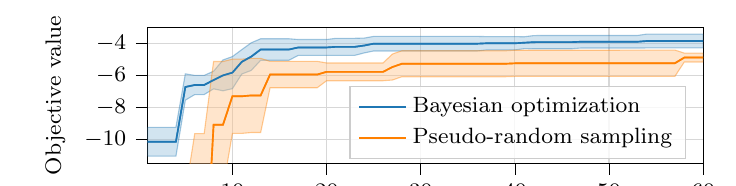
\begin{tikzpicture}[x=1in,y=1in]
  \useasboundingbox (-0.6, 0) rectangle (2.8, -0.65); %
    
  \definecolor{darkgrey176}{RGB}{176,176,176}
  \definecolor{lightgrey204}{RGB}{204,204,204}
  \definecolor{steelblue31119180}{RGB}{31,119,180}

  \begin{axis}[
  anchor=north west,
  width=3.4in,
  height=1.3in,
  legend cell align={left},
  legend style={
    fill opacity=0.8,
    draw opacity=1,
    text opacity=1,
    at={(0.97,0.03)},
    anchor=south east,
    font=\footnotesize,
    draw=lightgrey204
  },
  tick align=outside,
  tick pos=left,
  x grid style={darkgrey176!50},
  xlabel={Episodes},
  xmajorgrids,
  xmin=1, xmax=60,
  xtick style={color=black},
  y grid style={darkgrey176!50},
  ylabel={Objective value},
  ymajorgrids,
  xlabel shift=-1mm,
  ymin=-11.5, ymax=-3.0,
  ytick style={color=black},
  tick label style={font=\footnotesize}, %
  label style={font=\footnotesize}, %
  ]

  \addplot [semithick, steelblue31119180]
  table {%
  1 -10.1574191633144
  2 -10.1574191633144
  3 -10.1574191633144
  4 -10.1574191633144
  5 -6.72289483906331
  6 -6.59684858181106
  7 -6.59684858181106
  8 -6.28596903298211
  9 -5.99373655494911
  10 -5.82167779703389
  11 -5.1428110983115
  12 -4.81673457286373
  13 -4.37088875274734
  14 -4.37088875274734
  15 -4.37088875274734
  16 -4.37088875274734
  17 -4.24148141205882
  18 -4.24148141205882
  19 -4.24148141205882
  20 -4.24148141205882
  21 -4.20245990000189
  22 -4.20245990000189
  23 -4.20245990000189
  24 -4.11959725018268
  25 -4.00556881763445
  26 -4.00556881763445
  27 -4.00556881763445
  28 -4.00556881763445
  29 -4.00556881763445
  30 -4.00556881763445
  31 -4.00556881763445
  32 -4.00556881763445
  33 -4.00556881763445
  34 -4.00556881763445
  35 -4.00556881763445
  36 -4.00556881763445
  37 -3.97949251478588
  38 -3.97949251478588
  39 -3.97949251478588
  40 -3.97949251478588
  41 -3.94404729277079
  42 -3.91049026608397
  43 -3.90720589167441
  44 -3.90720589167441
  45 -3.90720589167441
  46 -3.90720589167441
  47 -3.88429011242476
  48 -3.88429011242476
  49 -3.88429011242476
  50 -3.88429011242476
  51 -3.88429011242476
  52 -3.88429011242476
  53 -3.88429011242476
  54 -3.83778249975218
  55 -3.83778249975218
  56 -3.83778249975218
  57 -3.83778249975218
  58 -3.83778249975218
  59 -3.83778249975218
  60 -3.83778249975218
  };
  \addlegendentry{Bayesian optimization}

  \path [draw=steelblue31119180!100, fill=steelblue31119180!50, opacity=0.4]
  (axis cs:1,-9.25192272947796)
  --(axis cs:1,-11.0629155971508)
  --(axis cs:2,-11.0629155971508)
  --(axis cs:3,-11.0629155971508)
  --(axis cs:4,-11.0629155971508)
  --(axis cs:5,-7.54939492206937)
  --(axis cs:6,-7.19721439515581)
  --(axis cs:7,-7.19721439515581)
  --(axis cs:8,-6.8386905924942)
  --(axis cs:9,-6.96114920237258)
  --(axis cs:10,-6.82854865024866)
  --(axis cs:11,-5.90839733741554)
  --(axis cs:12,-5.68382706642718)
  --(axis cs:13,-5.04568387720924)
  --(axis cs:14,-5.04568387720924)
  --(axis cs:15,-5.04568387720924)
  --(axis cs:16,-5.04568387720924)
  --(axis cs:17,-4.73792464284913)
  --(axis cs:18,-4.73792464284913)
  --(axis cs:19,-4.73792464284913)
  --(axis cs:20,-4.73792464284913)
  --(axis cs:21,-4.73733099029819)
  --(axis cs:22,-4.73733099029819)
  --(axis cs:23,-4.73733099029819)
  --(axis cs:24,-4.58459002120253)
  --(axis cs:25,-4.46280980134367)
  --(axis cs:26,-4.46280980134367)
  --(axis cs:27,-4.46280980134367)
  --(axis cs:28,-4.46280980134367)
  --(axis cs:29,-4.46280980134367)
  --(axis cs:30,-4.46280980134367)
  --(axis cs:31,-4.46280980134367)
  --(axis cs:32,-4.46280980134367)
  --(axis cs:33,-4.46280980134367)
  --(axis cs:34,-4.46280980134367)
  --(axis cs:35,-4.46280980134367)
  --(axis cs:36,-4.46280980134367)
  --(axis cs:37,-4.39831635351107)
  --(axis cs:38,-4.39831635351107)
  --(axis cs:39,-4.39831635351107)
  --(axis cs:40,-4.39831635351107)
  --(axis cs:41,-4.31605252044889)
  --(axis cs:42,-4.32412394230932)
  --(axis cs:43,-4.32527023808848)
  --(axis cs:44,-4.32527023808848)
  --(axis cs:45,-4.32527023808848)
  --(axis cs:46,-4.32527023808848)
  --(axis cs:47,-4.27735676012639)
  --(axis cs:48,-4.27735676012639)
  --(axis cs:49,-4.27735676012639)
  --(axis cs:50,-4.27735676012639)
  --(axis cs:51,-4.27735676012639)
  --(axis cs:52,-4.27735676012639)
  --(axis cs:53,-4.27735676012639)
  --(axis cs:54,-4.27143218019298)
  --(axis cs:55,-4.27143218019298)
  --(axis cs:56,-4.27143218019298)
  --(axis cs:57,-4.27143218019298)
  --(axis cs:58,-4.27143218019298)
  --(axis cs:59,-4.27143218019298)
  --(axis cs:60,-4.27143218019298)
  --(axis cs:60,-3.40413281931137)
  --(axis cs:60,-3.40413281931137)
  --(axis cs:59,-3.40413281931137)
  --(axis cs:58,-3.40413281931137)
  --(axis cs:57,-3.40413281931137)
  --(axis cs:56,-3.40413281931137)
  --(axis cs:55,-3.40413281931137)
  --(axis cs:54,-3.40413281931137)
  --(axis cs:53,-3.49122346472314)
  --(axis cs:52,-3.49122346472314)
  --(axis cs:51,-3.49122346472314)
  --(axis cs:50,-3.49122346472314)
  --(axis cs:49,-3.49122346472314)
  --(axis cs:48,-3.49122346472314)
  --(axis cs:47,-3.49122346472314)
  --(axis cs:46,-3.48914154526035)
  --(axis cs:45,-3.48914154526035)
  --(axis cs:44,-3.48914154526035)
  --(axis cs:43,-3.48914154526035)
  --(axis cs:42,-3.49685658985863)
  --(axis cs:41,-3.57204206509268)
  --(axis cs:40,-3.56066867606069)
  --(axis cs:39,-3.56066867606069)
  --(axis cs:38,-3.56066867606069)
  --(axis cs:37,-3.56066867606069)
  --(axis cs:36,-3.54832783392523)
  --(axis cs:35,-3.54832783392523)
  --(axis cs:34,-3.54832783392523)
  --(axis cs:33,-3.54832783392523)
  --(axis cs:32,-3.54832783392523)
  --(axis cs:31,-3.54832783392523)
  --(axis cs:30,-3.54832783392523)
  --(axis cs:29,-3.54832783392523)
  --(axis cs:28,-3.54832783392523)
  --(axis cs:27,-3.54832783392523)
  --(axis cs:26,-3.54832783392523)
  --(axis cs:25,-3.54832783392523)
  --(axis cs:24,-3.65460447916283)
  --(axis cs:23,-3.6675888097056)
  --(axis cs:22,-3.6675888097056)
  --(axis cs:21,-3.6675888097056)
  --(axis cs:20,-3.74503818126851)
  --(axis cs:19,-3.74503818126851)
  --(axis cs:18,-3.74503818126851)
  --(axis cs:17,-3.74503818126851)
  --(axis cs:16,-3.69609362828544)
  --(axis cs:15,-3.69609362828544)
  --(axis cs:14,-3.69609362828544)
  --(axis cs:13,-3.69609362828544)
  --(axis cs:12,-3.94964207930029)
  --(axis cs:11,-4.37722485920747)
  --(axis cs:10,-4.81480694381912)
  --(axis cs:9,-5.02632390752564)
  --(axis cs:8,-5.73324747347001)
  --(axis cs:7,-5.99648276846631)
  --(axis cs:6,-5.99648276846631)
  --(axis cs:5,-5.89639475605725)
  --(axis cs:4,-9.25192272947796)
  --(axis cs:3,-9.25192272947796)
  --(axis cs:2,-9.25192272947796)
  --(axis cs:1,-9.25192272947796)
  --cycle;

  \addplot [semithick, orange]
  table {%
  1 -24.8117548316848
  2 -24.8117548316848
  3 -24.8117548316848
  4 -24.8117548316848
  5 -23.9097738609303
  6 -20.0768245547915
  7 -20.0768245547915
  8 -9.09489985281767
  9 -9.09489985281767
  10 -7.30449400207115
  11 -7.30449400207115
  12 -7.25275367414012
  13 -7.25275367414012
  14 -5.94324016597094
  15 -5.94324016597094
  16 -5.94324016597094
  17 -5.94324016597094
  18 -5.94324016597094
  19 -5.94324016597094
  20 -5.77141780882547
  21 -5.77141780882547
  22 -5.77141780882547
  23 -5.77141780882547
  24 -5.77141780882547
  25 -5.77141780882547
  26 -5.77141780882547
  27 -5.46955325648097
  28 -5.26388748129056
  29 -5.26388748129056
  30 -5.26388748129056
  31 -5.26388748129056
  32 -5.26388748129056
  33 -5.26388748129056
  34 -5.26388748129056
  35 -5.26388748129056
  36 -5.26388748129056
  37 -5.26388748129056
  38 -5.26388748129056
  39 -5.26388748129056
  40 -5.23696661156889
  41 -5.23696661156889
  42 -5.23696661156889
  43 -5.23696661156889
  44 -5.23696661156889
  45 -5.23696661156889
  46 -5.23696661156889
  47 -5.23696661156889
  48 -5.23696661156889
  49 -5.23696661156889
  50 -5.23696661156889
  51 -5.23696661156889
  52 -5.22987952313497
  53 -5.22987952313497
  54 -5.22987952313497
  55 -5.22987952313497
  56 -5.22987952313497
  57 -5.22987952313497
  58 -4.8758610705042
  59 -4.8758610705042
  60 -4.8758610705042
  };
  \addlegendentry{Pseudo-random sampling}

  \path [draw=orange!100, fill=orange!50, opacity=0.4]
  (axis cs:1,-15.8254505980391)
  --(axis cs:1,-33.7980590653305)
  --(axis cs:2,-33.7980590653305)
  --(axis cs:3,-33.7980590653305)
  --(axis cs:4,-33.7980590653305)
  --(axis cs:5,-34.4583549633831)
  --(axis cs:6,-30.500835698174)
  --(axis cs:7,-30.500835698174)
  --(axis cs:8,-13.0650976691005)
  --(axis cs:9,-13.0650976691005)
  --(axis cs:10,-9.63305186269427)
  --(axis cs:11,-9.63305186269427)
  --(axis cs:12,-9.57854407058712)
  --(axis cs:13,-9.57854407058712)
  --(axis cs:14,-6.7726501658824)
  --(axis cs:15,-6.7726501658824)
  --(axis cs:16,-6.7726501658824)
  --(axis cs:17,-6.7726501658824)
  --(axis cs:18,-6.7726501658824)
  --(axis cs:19,-6.7726501658824)
  --(axis cs:20,-6.32853325564196)
  --(axis cs:21,-6.32853325564196)
  --(axis cs:22,-6.32853325564196)
  --(axis cs:23,-6.32853325564196)
  --(axis cs:24,-6.32853325564196)
  --(axis cs:25,-6.32853325564196)
  --(axis cs:26,-6.32853325564196)
  --(axis cs:27,-6.28418882407104)
  --(axis cs:28,-6.07760333508252)
  --(axis cs:29,-6.07760333508252)
  --(axis cs:30,-6.07760333508252)
  --(axis cs:31,-6.07760333508252)
  --(axis cs:32,-6.07760333508252)
  --(axis cs:33,-6.07760333508252)
  --(axis cs:34,-6.07760333508252)
  --(axis cs:35,-6.07760333508252)
  --(axis cs:36,-6.07760333508252)
  --(axis cs:37,-6.07760333508252)
  --(axis cs:38,-6.07760333508252)
  --(axis cs:39,-6.07760333508252)
  --(axis cs:40,-6.05896797065684)
  --(axis cs:41,-6.05896797065684)
  --(axis cs:42,-6.05896797065684)
  --(axis cs:43,-6.05896797065684)
  --(axis cs:44,-6.05896797065684)
  --(axis cs:45,-6.05896797065684)
  --(axis cs:46,-6.05896797065684)
  --(axis cs:47,-6.05896797065684)
  --(axis cs:48,-6.05896797065684)
  --(axis cs:49,-6.05896797065684)
  --(axis cs:50,-6.05896797065684)
  --(axis cs:51,-6.05896797065684)
  --(axis cs:52,-6.05436508485352)
  --(axis cs:53,-6.05436508485352)
  --(axis cs:54,-6.05436508485352)
  --(axis cs:55,-6.05436508485352)
  --(axis cs:56,-6.05436508485352)
  --(axis cs:57,-6.05436508485352)
  --(axis cs:58,-5.15323923666181)
  --(axis cs:59,-5.15323923666181)
  --(axis cs:60,-5.15323923666181)
  --(axis cs:60,-4.59848290434659)
  --(axis cs:60,-4.59848290434659)
  --(axis cs:59,-4.59848290434659)
  --(axis cs:58,-4.59848290434659)
  --(axis cs:57,-4.40539396141641)
  --(axis cs:56,-4.40539396141641)
  --(axis cs:55,-4.40539396141641)
  --(axis cs:54,-4.40539396141641)
  --(axis cs:53,-4.40539396141641)
  --(axis cs:52,-4.40539396141641)
  --(axis cs:51,-4.41496525248093)
  --(axis cs:50,-4.41496525248093)
  --(axis cs:49,-4.41496525248093)
  --(axis cs:48,-4.41496525248093)
  --(axis cs:47,-4.41496525248093)
  --(axis cs:46,-4.41496525248093)
  --(axis cs:45,-4.41496525248093)
  --(axis cs:44,-4.41496525248093)
  --(axis cs:43,-4.41496525248093)
  --(axis cs:42,-4.41496525248093)
  --(axis cs:41,-4.41496525248093)
  --(axis cs:40,-4.41496525248093)
  --(axis cs:39,-4.45017162749861)
  --(axis cs:38,-4.45017162749861)
  --(axis cs:37,-4.45017162749861)
  --(axis cs:36,-4.45017162749861)
  --(axis cs:35,-4.45017162749861)
  --(axis cs:34,-4.45017162749861)
  --(axis cs:33,-4.45017162749861)
  --(axis cs:32,-4.45017162749861)
  --(axis cs:31,-4.45017162749861)
  --(axis cs:30,-4.45017162749861)
  --(axis cs:29,-4.45017162749861)
  --(axis cs:28,-4.45017162749861)
  --(axis cs:27,-4.65491768889089)
  --(axis cs:26,-5.21430236200899)
  --(axis cs:25,-5.21430236200899)
  --(axis cs:24,-5.21430236200899)
  --(axis cs:23,-5.21430236200899)
  --(axis cs:22,-5.21430236200899)
  --(axis cs:21,-5.21430236200899)
  --(axis cs:20,-5.21430236200899)
  --(axis cs:19,-5.11383016605948)
  --(axis cs:18,-5.11383016605948)
  --(axis cs:17,-5.11383016605948)
  --(axis cs:16,-5.11383016605948)
  --(axis cs:15,-5.11383016605948)
  --(axis cs:14,-5.11383016605948)
  --(axis cs:13,-4.92696327769312)
  --(axis cs:12,-4.92696327769312)
  --(axis cs:11,-4.97593614144803)
  --(axis cs:10,-4.97593614144803)
  --(axis cs:9,-5.12470203653484)
  --(axis cs:8,-5.12470203653484)
  --(axis cs:7,-9.65281341140902)
  --(axis cs:6,-9.65281341140902)
  --(axis cs:5,-13.3611927584774)
  --(axis cs:4,-15.8254505980391)
  --(axis cs:3,-15.8254505980391)
  --(axis cs:2,-15.8254505980391)
  --(axis cs:1,-15.8254505980391)
  --cycle;


  \addplot [semithick, steelblue31119180]
  table {%
  1 -10.1574191633144
  2 -10.1574191633144
  3 -10.1574191633144
  4 -10.1574191633144
  5 -6.72289483906331
  6 -6.59684858181106
  7 -6.59684858181106
  8 -6.28596903298211
  9 -5.99373655494911
  10 -5.82167779703389
  11 -5.1428110983115
  12 -4.81673457286373
  13 -4.37088875274734
  14 -4.37088875274734
  15 -4.37088875274734
  16 -4.37088875274734
  17 -4.24148141205882
  18 -4.24148141205882
  19 -4.24148141205882
  20 -4.24148141205882
  21 -4.20245990000189
  22 -4.20245990000189
  23 -4.20245990000189
  24 -4.11959725018268
  25 -4.00556881763445
  26 -4.00556881763445
  27 -4.00556881763445
  28 -4.00556881763445
  29 -4.00556881763445
  30 -4.00556881763445
  31 -4.00556881763445
  32 -4.00556881763445
  33 -4.00556881763445
  34 -4.00556881763445
  35 -4.00556881763445
  36 -4.00556881763445
  37 -3.97949251478588
  38 -3.97949251478588
  39 -3.97949251478588
  40 -3.97949251478588
  41 -3.94404729277079
  42 -3.91049026608397
  43 -3.90720589167441
  44 -3.90720589167441
  45 -3.90720589167441
  46 -3.90720589167441
  47 -3.88429011242476
  48 -3.88429011242476
  49 -3.88429011242476
  50 -3.88429011242476
  51 -3.88429011242476
  52 -3.88429011242476
  53 -3.88429011242476
  54 -3.83778249975218
  55 -3.83778249975218
  56 -3.83778249975218
  57 -3.83778249975218
  58 -3.83778249975218
  59 -3.83778249975218
  60 -3.83778249975218
  };
  


  \addplot [semithick, orange]
  table {%
  1 -24.8117548316848
  2 -24.8117548316848
  3 -24.8117548316848
  4 -24.8117548316848
  5 -23.9097738609303
  6 -20.0768245547915
  7 -20.0768245547915
  8 -9.09489985281767
  9 -9.09489985281767
  10 -7.30449400207115
  11 -7.30449400207115
  12 -7.25275367414012
  13 -7.25275367414012
  14 -5.94324016597094
  15 -5.94324016597094
  16 -5.94324016597094
  17 -5.94324016597094
  18 -5.94324016597094
  19 -5.94324016597094
  20 -5.77141780882547
  21 -5.77141780882547
  22 -5.77141780882547
  23 -5.77141780882547
  24 -5.77141780882547
  25 -5.77141780882547
  26 -5.77141780882547
  27 -5.46955325648097
  28 -5.26388748129056
  29 -5.26388748129056
  30 -5.26388748129056
  31 -5.26388748129056
  32 -5.26388748129056
  33 -5.26388748129056
  34 -5.26388748129056
  35 -5.26388748129056
  36 -5.26388748129056
  37 -5.26388748129056
  38 -5.26388748129056
  39 -5.26388748129056
  40 -5.23696661156889
  41 -5.23696661156889
  42 -5.23696661156889
  43 -5.23696661156889
  44 -5.23696661156889
  45 -5.23696661156889
  46 -5.23696661156889
  47 -5.23696661156889
  48 -5.23696661156889
  49 -5.23696661156889
  50 -5.23696661156889
  51 -5.23696661156889
  52 -5.22987952313497
  53 -5.22987952313497
  54 -5.22987952313497
  55 -5.22987952313497
  56 -5.22987952313497
  57 -5.22987952313497
  58 -4.8758610705042
  59 -4.8758610705042
  60 -4.8758610705042
  };
  
  
  \addplot [very thick, black, dash pattern=on 11.1pt off 4.8pt]
  table {%
  0 0
  59 0
  };
  \end{axis}

  \end{tikzpicture}

    \caption{Performance of the best controller found by BO ({\color{blue}blue}) for a given number of trials (episodes) compared to a pseudo-random baseline ({\color{orange}orange}). Intervals are the standard deviation over five random seeds.}
    \label{fig:boperformanceimprovement}
\end{figure}


\subsection{Fast Neural Network Approximate MPC}
\label{sec:ampc}
Despite great engineering efforts, nonlinear solvers still struggle to solve MPC optimization problems in real-time on embedded CPUs.
Instead, we use imitation learning to find an explicit mapping from states to actions in the form of a neural network that approximates the MPC described in Section~\ref{sec:nonlinearmpc}.
The approximate MPC is several orders of magnitude faster (onboard inference in less than~\SI{300}{\micro\second}) compared to solving the optimization problem~\eqref{eqn:mpc}, which takes several hundred milliseconds on a desktop CPU.
It thus allows a sophisticated nonlinear MPC with convoluted system dynamics, fine discretization, and a long prediction horizon to run onboard the robot.
With this, we achieve -- for the first time -- articulated driving following high level yaw and velocity setpoints, e.g., provided by keyboard.

We imitate the optimal solution to~(\ref{eqn:mpc}) by first sampling a large dataset of random states~$x$ and optimal solutions~$u^*(x)$ containing \num{3.5} million points.
We use a multi-layer perceptron with \num{4} layers, \num{100} neurons per layer, and a mixture of tangent hyperbolic and rectified linear activations as function approximator, which is trained in Jax.
To achieve fast control, we implement inference in C++ using Eigen onboard the Mini Wheelbot.
The final controller on the Mini Wheelbot hardware driving around based on keyboard heading and velocity commands is shown in Fig.~\ref{fig:mpcexperiments} and the supplementary video.
This is the first time that controlled driving along specified directions is achieved for a reaction wheel balancing unicycle of this kind.

\begin{figure}[tb]
    \newcommand{\photoheight}{1.2in}
    \newcommand{\plotwidth}{1.65in}
    \newcommand{\plotheight}{1.4in}
    \centering
    \begin{subfigure}[t]{1.6in}
        \centering
        \includegraphics[height=\photoheight,trim=0.5in 0 0.5in 0, clip]{figures/yaw-control-plot/overlay_driving_3.jpg}
    \end{subfigure}
    \begin{subfigure}[t]{1.6in}
        \centering
        \begin{tikzpicture}
    \node[anchor=south west,inner sep=0] (image) at (0,0) {\includegraphics[height=\photoheight]{figures/yaw-control-plot/photos/mosaic_wb.jpg}};
    \begin{scope}[x={(image.south east)},y={(image.north west)}, font=\tiny]
        \coordinate (A_label) at (0.07,0.92);
        \coordinate (B_label) at (0.57,0.92);
        \coordinate (C_label) at (0.57,0.41);
        \coordinate (D_label) at (0.07,0.41);
        
        \draw[->,thick,black] (0.4,0.72) -- ++(0,0) -- (0.6,0.72) node[midway, above] {rot. 90°};
        \draw[->,thick,black] (0.75,0.6) -- ++(0,0) -- (0.75,0.4) node[midway, above right, yshift=-0.5mm, xshift=-0.5mm]{rot. 90°};
        \draw[->,thick,black] (0.6,0.27) -- ++(0,0) -- (0.4,0.27) node[midway,below] {rot. 90°};

    \end{scope}
\end{tikzpicture}

    \end{subfigure}
    \par\medskip %
    \begin{subfigure}[t]{1.4in}
        \centering
        \begin{tikzpicture}[x=1in, y=1in,spy using outlines={circle, magnification=4, connect spies}]
  \useasboundingbox (-0.90, 0.1) rectangle (0.7, -0.85); %
    \definecolor{darkgray100}{RGB}{100,100,100}
    \definecolor{darkgray176}{RGB}{176,176,176}
    \definecolor{lightgray204}{RGB}{204,204,204}
    


    


    
    
    
    


    \begin{axis}[
        name=other,
        xshift=0mm,
        anchor=north,
        ytick distance = 0.2,
        xtick distance = 0.2,
        ytick style={color=black},
        ymajorgrids,
        ymin=-0.3, ymax=0.1,
        xmin=-0.2, xmax=0.2,
        y label style={yshift=-2mm},
        x label style={yshift=2mm},
        x grid style={darkgray176},
        xmajorgrids,
        xtick style={color=black},
        y grid style={darkgray176},
        ylabel={{Pos. y [m]}},
        xlabel={{Pos. x [m]}},
        label style={font=\scriptsize},
        ticklabel style={font=\scriptsize},
        height=\plotheight,
        legend style={
            fill opacity=1,
            draw opacity=1,
            text opacity=1,
            at={(1.02, -0.05)},
            anchor=south east,
            font=\scriptsize,
            draw=lightgray204
          },
        reverse legend,
        axis equal
        ]


    


    
    \addplot[thick, color=blue] table [x=x, y=y, col sep=comma] {figures/yaw-control-plot/yaw_tracking_error.csv};
    
    
    

    \end{axis}


    
        
    
        
    
    
        
    
    \end{tikzpicture}

    \end{subfigure}\hspace{0.2in}
    \begin{subfigure}[t]{1.6in}
        
\begin{tikzpicture}[x=1in,y=1in]
  \useasboundingbox (-0.80, 0.1) rectangle (0.8, -0.85); %
    \definecolor{darkgray100}{RGB}{100,100,100}
    \definecolor{darkgray176}{RGB}{176,176,176}
    \definecolor{lightgray204}{RGB}{204,204,204}
    
        \begin{axis}[
            name=yaw,
            anchor=north,
            ytick style={color=black},
            ytick={-1.57, 0, 1.57},
            yticklabels={-$\frac{\pi}{2}$, $0$, $\frac{\pi}{2}$},
            ymajorgrids,
            ymin=-2, ymax=2,
            y label style={yshift=-2mm},
            x grid style={darkgray176},
            xmajorgrids,
            xmin=0, xmax=22,
            xtick style={color=black},
            y grid style={darkgray176},
            x label style={yshift=2mm},
            xlabel={Time [s]},
            ylabel={{Yaw $\psi$ [rad]}},
            height=\plotheight, width=\plotwidth,
            label style={font=\scriptsize},
            ticklabel style={font=\scriptsize},
            legend cell align={left},
            legend style={
              draw opacity=1,
              text opacity=1,
              at={(1.25,1.1)},
              anchor=north east,
              draw=lightgray204,
              font=\scriptsize
            },
            reverse legend,
        ]
    
        \addplot[mark=none, thick, color=darkgray100] table [x=time, y=yaw_setpoint, col sep=comma] {figures/yaw-control-plot/wheelbot_hardware_turbo_initial.csv};
        \addlegendentry{Reference};
    
        
    
        \addplot[mark=none, thick, color=blue] table [x=time, y=yaw, col sep=comma] {figures/yaw-control-plot/wheelbot_hardware_turbo_initial.csv};
        \addlegendentry{Measured};
    
        
        \end{axis}
    \end{tikzpicture}

    \end{subfigure}
    \caption{Approximate MPC experiments: Driving around based on keyboard heading and velocity commands (left) and yaw reference step response (right).
    The controller runs onboard the Mini Wheelbot.
    }
    \label{fig:mpcexperiments}
\end{figure}
